\documentclass[conference]{IEEEtran}
%DIF LATEXDIFF DIFFERENCE FILE
%DIF DEL ieee-initial-version.tex       Sun May 18 16:05:00 2025
%DIF ADD ieee-most-recent-version.tex   Sun May 18 15:56:32 2025
\usepackage[utf8]{inputenc}

\IEEEoverridecommandlockouts
%DIF 5c5
%DIF < % The preceding line is only needed to identify funding in the first footnote. If that is unneeded, please comment it out.
%DIF -------
 %DIF > 
%DIF -------
\usepackage{cite}
\usepackage{amsmath,amssymb,amsfonts}
\usepackage{algorithmic}
\usepackage{graphicx}
\usepackage{textcomp}
\usepackage{xcolor}
\usepackage{multirow}
\usepackage{tikz}
%DIF 14a14
\usetikzlibrary{positioning} %DIF > 
%DIF -------
\def\checkmark{\tikz\fill[scale=0.4](0,.35) -- (.25,0) -- (1,.7) -- (.25,.15) -- cycle;}
%DIF 15d16
%DIF < \usepackage{graphicx}
%DIF -------
\usepackage{svg}
\usepackage{listings}
%DIF 18-20d18
%DIF < %\def\BibTeX{{\rm B\kern-.05em{\sc i\kern-.025em b}\kern-.08em
%DIF < %    T\kern-.1667em\lower.7ex\hbox{E}\kern-.125emX}}
%DIF < \addtolength{\topmargin}{+0.1cm} % had to add this to be able to submit to EDAS, don't touch
%DIF -------

%DIF 22-26c19-24
%DIF < %\usepackage[
%DIF < %backend=biber,
%DIF < %style=alphabetic,
%DIF < %sorting=ynt
%DIF < %]{biblatex}
%DIF -------
%colours %DIF > 
\definecolor{pastelblue1}{HTML}{B0D0D3} % Powder Blue %DIF > 
\definecolor{pastelblue2}{HTML}{C7D2FE} % Periwinkle Mist %DIF > 
\definecolor{pastelblue3}{HTML}{D4E8F4} % Sky Whisper %DIF > 
\definecolor{pastelblue4}{HTML}{A8C5DA} % Arctic Haze %DIF > 
\definecolor{pastelblue5}{HTML}{C3CFE2} % Frosted Indigo %DIF > 
%DIF -------

%DIF 28a26-27
\addtolength{\topmargin}{+0.1cm}  %DIF > 
 %DIF > 
%DIF -------
\lstdefinelanguage{json}{
    basicstyle=\ttfamily\footnotesize,
    breaklines=true,
    morestring=[b]",
    morecomment=[l]{//},
}
%DIF < 
%DIF < %\addbibresource{bibliography.bib}  
%DIF PREAMBLE EXTENSION ADDED BY LATEXDIFF
%DIF UNDERLINE PREAMBLE %DIF PREAMBLE
\RequirePackage[normalem]{ulem} %DIF PREAMBLE
\RequirePackage{color}\definecolor{RED}{rgb}{1,0,0}\definecolor{BLUE}{rgb}{0,0,1} %DIF PREAMBLE
\providecommand{\DIFadd}[1]{{\protect\color{blue}\uwave{#1}}} %DIF PREAMBLE
\providecommand{\DIFdel}[1]{{\protect\color{red}\sout{#1}}} %DIF PREAMBLE
%DIF SAFE PREAMBLE %DIF PREAMBLE
\providecommand{\DIFaddbegin}{} %DIF PREAMBLE
\providecommand{\DIFaddend}{} %DIF PREAMBLE
\providecommand{\DIFdelbegin}{} %DIF PREAMBLE
\providecommand{\DIFdelend}{} %DIF PREAMBLE
\providecommand{\DIFmodbegin}{} %DIF PREAMBLE
\providecommand{\DIFmodend}{} %DIF PREAMBLE
%DIF FLOATSAFE PREAMBLE %DIF PREAMBLE
\providecommand{\DIFaddFL}[1]{\DIFadd{#1}} %DIF PREAMBLE
\providecommand{\DIFdelFL}[1]{\DIFdel{#1}} %DIF PREAMBLE
\providecommand{\DIFaddbeginFL}{} %DIF PREAMBLE
\providecommand{\DIFaddendFL}{} %DIF PREAMBLE
\providecommand{\DIFdelbeginFL}{} %DIF PREAMBLE
\providecommand{\DIFdelendFL}{} %DIF PREAMBLE
\newcommand{\DIFscaledelfig}{0.5}
%DIF HIGHLIGHTGRAPHICS PREAMBLE %DIF PREAMBLE
\RequirePackage{settobox} %DIF PREAMBLE
\RequirePackage{letltxmacro} %DIF PREAMBLE
\newsavebox{\DIFdelgraphicsbox} %DIF PREAMBLE
\newlength{\DIFdelgraphicswidth} %DIF PREAMBLE
\newlength{\DIFdelgraphicsheight} %DIF PREAMBLE
% store original definition of \includegraphics %DIF PREAMBLE
\LetLtxMacro{\DIFOincludegraphics}{\includegraphics} %DIF PREAMBLE
\newcommand{\DIFaddincludegraphics}[2][]{{\color{blue}\fbox{\DIFOincludegraphics[#1]{#2}}}} %DIF PREAMBLE
\newcommand{\DIFdelincludegraphics}[2][]{% %DIF PREAMBLE
\sbox{\DIFdelgraphicsbox}{\DIFOincludegraphics[#1]{#2}}% %DIF PREAMBLE
\settoboxwidth{\DIFdelgraphicswidth}{\DIFdelgraphicsbox} %DIF PREAMBLE
\settoboxtotalheight{\DIFdelgraphicsheight}{\DIFdelgraphicsbox} %DIF PREAMBLE
\scalebox{\DIFscaledelfig}{% %DIF PREAMBLE
\parbox[b]{\DIFdelgraphicswidth}{\usebox{\DIFdelgraphicsbox}\\[-\baselineskip] \rule{\DIFdelgraphicswidth}{0em}}\llap{\resizebox{\DIFdelgraphicswidth}{\DIFdelgraphicsheight}{% %DIF PREAMBLE
\setlength{\unitlength}{\DIFdelgraphicswidth}% %DIF PREAMBLE
\begin{picture}(1,1)% %DIF PREAMBLE
\thicklines\linethickness{2pt} %DIF PREAMBLE
{\color[rgb]{1,0,0}\put(0,0){\framebox(1,1){}}}% %DIF PREAMBLE
{\color[rgb]{1,0,0}\put(0,0){\line( 1,1){1}}}% %DIF PREAMBLE
{\color[rgb]{1,0,0}\put(0,1){\line(1,-1){1}}}% %DIF PREAMBLE
\end{picture}% %DIF PREAMBLE
}\hspace*{3pt}}} %DIF PREAMBLE
} %DIF PREAMBLE
\LetLtxMacro{\DIFOaddbegin}{\DIFaddbegin} %DIF PREAMBLE
\LetLtxMacro{\DIFOaddend}{\DIFaddend} %DIF PREAMBLE
\LetLtxMacro{\DIFOdelbegin}{\DIFdelbegin} %DIF PREAMBLE
\LetLtxMacro{\DIFOdelend}{\DIFdelend} %DIF PREAMBLE
\DeclareRobustCommand{\DIFaddbegin}{\DIFOaddbegin \let\includegraphics\DIFaddincludegraphics} %DIF PREAMBLE
\DeclareRobustCommand{\DIFaddend}{\DIFOaddend \let\includegraphics\DIFOincludegraphics} %DIF PREAMBLE
\DeclareRobustCommand{\DIFdelbegin}{\DIFOdelbegin \let\includegraphics\DIFdelincludegraphics} %DIF PREAMBLE
\DeclareRobustCommand{\DIFdelend}{\DIFOaddend \let\includegraphics\DIFOincludegraphics} %DIF PREAMBLE
\LetLtxMacro{\DIFOaddbeginFL}{\DIFaddbeginFL} %DIF PREAMBLE
\LetLtxMacro{\DIFOaddendFL}{\DIFaddendFL} %DIF PREAMBLE
\LetLtxMacro{\DIFOdelbeginFL}{\DIFdelbeginFL} %DIF PREAMBLE
\LetLtxMacro{\DIFOdelendFL}{\DIFdelendFL} %DIF PREAMBLE
\DeclareRobustCommand{\DIFaddbeginFL}{\DIFOaddbeginFL \let\includegraphics\DIFaddincludegraphics} %DIF PREAMBLE
\DeclareRobustCommand{\DIFaddendFL}{\DIFOaddendFL \let\includegraphics\DIFOincludegraphics} %DIF PREAMBLE
\DeclareRobustCommand{\DIFdelbeginFL}{\DIFOdelbeginFL \let\includegraphics\DIFdelincludegraphics} %DIF PREAMBLE
\DeclareRobustCommand{\DIFdelendFL}{\DIFOaddendFL \let\includegraphics\DIFOincludegraphics} %DIF PREAMBLE
%DIF AMSMATHULEM PREAMBLE %DIF PREAMBLE
\makeatletter %DIF PREAMBLE
\let\sout@orig\sout %DIF PREAMBLE
\renewcommand{\sout}[1]{\ifmmode\text{\sout@orig{\ensuremath{#1}}}\else\sout@orig{#1}\fi} %DIF PREAMBLE
\makeatother %DIF PREAMBLE
%DIF COLORLISTINGS PREAMBLE %DIF PREAMBLE
\RequirePackage{listings} %DIF PREAMBLE
\RequirePackage{color} %DIF PREAMBLE
\lstdefinelanguage{DIFcode}{ %DIF PREAMBLE
%DIF DIFCODE_UNDERLINE %DIF PREAMBLE
  moredelim=[il][\color{red}\sout]{\%DIF\ <\ }, %DIF PREAMBLE
  moredelim=[il][\color{blue}\uwave]{\%DIF\ >\ } %DIF PREAMBLE
} %DIF PREAMBLE
\lstdefinestyle{DIFverbatimstyle}{ %DIF PREAMBLE
	language=DIFcode, %DIF PREAMBLE
	basicstyle=\ttfamily, %DIF PREAMBLE
	columns=fullflexible, %DIF PREAMBLE
	keepspaces=true %DIF PREAMBLE
} %DIF PREAMBLE
\lstnewenvironment{DIFverbatim}{\lstset{style=DIFverbatimstyle}}{} %DIF PREAMBLE
\lstnewenvironment{DIFverbatim*}{\lstset{style=DIFverbatimstyle,showspaces=true}}{} %DIF PREAMBLE
\lstset{extendedchars=\true,inputencoding=utf8}

%DIF END PREAMBLE EXTENSION ADDED BY LATEXDIFF

\begin{document}

\title{Network Identity Management: Application, Action and Device \DIFdelbegin \DIFdel{‑}\DIFdelend Aware Monitoring }

\author{\IEEEauthorblockN{Cenab Batu Bora}
\IEEEauthorblockA{\textit{Faculty of Computing Science} \\
\textit{University of Alberta}\\
Edmonton, Canada \\
cenab@ualberta.ca}
\and
\IEEEauthorblockN{Julia Silva Weber}
\IEEEauthorblockA{\textit{Faculty of Computer Science} \\
\textit{Dalhousie University}\\
Halifax, Canada \\
julia.weber@dal.ca}
\and
\IEEEauthorblockN{Nur Zincir-Heywood}
\IEEEauthorblockA{ \textit{Faculty of Computer Science} \\
\textit{Dalhousie University}\\
Halifax, Canada \\
zincir@cs.dal.ca}
}

\maketitle



\begin{abstract}
%DIF < Enterprise networks face significant security and compliance challenges as employees utilize a wide range of encrypted mobile applications on their unsecured devices, often bypassing workplace policies and potentially leading to possible policy violations or data leakage. It is often impossible for current firewall-based tools to enforce fine-grained access control over application features based on user roles and permissions within encrypted mobile applications.
\DIFdelbegin \DIFdel{Instant Message applications }\DIFdelend \DIFaddbegin \DIFadd{Instant Message Applications }\DIFaddend (IMAs) are often used in sensitive environments\DIFaddbegin \DIFadd{, }\DIFaddend where they pose a significant risk of accidental policy breaches or security lapses. %DIF < For instance, the 2021 Apple iMessage zero-day vulnerability allowed attackers to deploy Pegasus spyware, compromising user privacy without any user interaction. 
\DIFdelbegin \DIFdel{This paper introduces techniques for }\DIFdelend \DIFaddbegin \DIFadd{To address these risks, this paper introduces }\DIFaddend Network Identity Management (NIM)\DIFdelbegin \DIFdel{targeting these high‑risk IMAs}\DIFdelend \DIFaddbegin \DIFadd{, a set of techniques specifically designed for such high-risk applications}\DIFaddend . NIM provides a novel approach that enables network-layer, identity-aware access control for encrypted applications. To \DIFdelbegin \DIFdel{provide }\DIFdelend \DIFaddbegin \DIFadd{support NIM, we introduce techniques to establish }\DIFaddend the essential visibility layer\DIFdelbegin \DIFdel{for NIM, this paper presents techniques grounded in MLanalysis of }\DIFdelend \DIFaddbegin \DIFadd{. These techniques use machine learning (ML) to analyze }\DIFaddend encrypted traffic metadata\DIFdelbegin \DIFdel{, trained using data from our scalable}\DIFdelend \DIFaddbegin \DIFadd{. The ML models are trained on data produced by our scalable, }\DIFaddend cloud-native Android traffic generation framework. Our ML framework accurately identifies: (1) the application in use, (2) the specific user action being performed, and (3) the originating device—using only encrypted traffic metadata from multi-user environments. \DIFdelbegin \DIFdel{With }\DIFdelend \DIFaddbegin \DIFadd{For its primary task, our method, using }\DIFaddend emulated traffic from eight \DIFdelbegin \DIFdel{IMAs for the primary task, our method achieves }\DIFdelend \DIFaddbegin \DIFadd{Instant Messaging Applications (IMAs), yielded }\DIFaddend a 98.6\% F1-score \DIFdelbegin \DIFdel{via Gradient Boosting }\DIFdelend for application identification \DIFdelbegin \DIFdel{and }\DIFdelend \DIFaddbegin \DIFadd{with Gradient Boosting. Additionally, the method demonstrated }\DIFaddend near-perfect device identification based \DIFdelbegin \DIFdel{solely }\DIFdelend \DIFaddbegin \DIFadd{exclusively }\DIFaddend on encrypted traffic metadata. Furthermore, supplementary experiments provide initial validation for user action classification (group vs. one‑on‑one messaging), achieving \DIFaddbegin \DIFadd{a }\DIFaddend 73.3\% F1-score in distinguishing between group chats and direct messages using environment-agnostic patterns. 
%DIF < Organizations can now tell which app and device each user or group is using. Combined with action-level visibility, this allows NIM to enforce policies proactively—before any misuse occurs—strengthening overall enterprise security.
\end{abstract}

\begin{IEEEkeywords}
Encrypted traffic analysis, instant messaging applications, AI/ML, network identity management 
\end{IEEEkeywords}

\section{Introduction}
The use of powerful, encrypted mobile applications, often on employee-owned devices (BYOD), is widespread in enterprise and government networks. \DIFdelbegin \DIFdel{While essential for productivity}\DIFdelend \DIFaddbegin \DIFadd{However}\DIFaddend , organizations must ensure \DIFdelbegin \DIFdel{these tools are used securely and compliantly, and must }\DIFdelend \DIFaddbegin \DIFadd{their secure and compliant use to }\DIFaddend prevent accidental data leakage or unauthorized user actions. Crucially, this must be achieved while upholding user privacy and the security benefits provided by end-to-end encryption. Traditional policy enforcement methods relying on firewalls, domain blocking, and traffic inspection are incompatible with modern encryption standards. \DIFdelbegin \DIFdel{This necessitates innovative }\DIFdelend \DIFaddbegin \DIFadd{Consequently, practical }\DIFaddend solutions like the proposed Network Identity Management (NIM) \DIFdelbegin \DIFdel{, which aims to infer activity, such as which app is }\DIFdelend \DIFaddbegin \DIFadd{are required. NIM is designed to infer key activities—such as the application }\DIFaddend being used, \DIFdelbegin \DIFdel{which device it is coming from and what kind of action is being taken, }\DIFdelend \DIFaddbegin \DIFadd{its device of origin, and the nature of the action (}\DIFaddend like a video call or group chat\DIFdelbegin \DIFdel{. Application, action, and device identities are inferred through traffic pattern analysis. }\DIFdelend \DIFaddbegin \DIFadd{)—based on network behavior. }\DIFaddend Based on this visibility, NIM can enforce granular, predefined permission levels or policies\DIFdelbegin \DIFdel{(e.g., restricting }\DIFdelend \DIFaddbegin \DIFadd{. For instance, it can restrict }\DIFaddend access to certain applications or high-risk features based on user roles\DIFdelbegin \DIFdel{) solely through }\DIFdelend \DIFaddbegin \DIFadd{. These enforcement actions rely solely on }\DIFaddend communication patterns and information from encrypted traffic. \DIFdelbegin \DIFdel{Instant Messaging Applications (IMAs) exemplify tools where such pattern-based, policy-driven control is needed to mitigate risks proactively, moving beyond ineffective or excessive measures}\DIFdelend \DIFaddbegin \DIFadd{This methodology represents a significant advancement over current measures, which are often ineffective or overly restrictive}\DIFaddend .

\DIFdelbegin \DIFdel{To address this, this paper introduces foundational techniques for NIM , envisioning }\DIFdelend \DIFaddbegin \DIFadd{NIM is conceptualized as }\DIFaddend a network-layer Identity and Access Management system for encrypted \DIFdelbegin \DIFdel{traffic. Similar in principle to Role-Based Access Control, NIM aims to make }\DIFdelend \DIFaddbegin \DIFadd{applications. NIM facilitates }\DIFaddend context-aware access decisions \DIFdelbegin \DIFdel{based on verified identity before granting }\DIFdelend \DIFaddbegin \DIFadd{through a deliberate sequence: it first validates user identity and then permits }\DIFaddend network access to \DIFdelbegin \DIFdel{specific applicationsand features. Such a system }\DIFdelend \DIFaddbegin \DIFadd{particular applications, a methodology akin to Role-Based Access Control. In this framework, NIM }\DIFaddend defines access groups based on organizational roles and \DIFaddbegin \DIFadd{then }\DIFaddend assigns permissions for specific applications or resources to these groups. When a device connects, it \DIFdelbegin \DIFdel{is linked to a useridentity and its associated }\DIFdelend \DIFaddbegin \DIFadd{becomes associated with a user's identity and their designated access }\DIFaddend group(s). The \DIFdelbegin \DIFdel{core challenge NIM addresses is discerning the application . %DIF < and potentially its features being accessed through the encrypted traffic to enforce these permissions.
}\DIFdelend \DIFaddbegin \DIFadd{fundamental technical challenge for NIM lies in reliably identifying the application solely from encrypted traffic data.
}\DIFaddend 

Our method analyzes encrypted traffic metadata to \DIFdelbegin \DIFdel{determine the application in use and the }\DIFdelend \DIFaddbegin \DIFadd{identify the active application and its }\DIFaddend source device. Furthermore, by \DIFdelbegin \DIFdel{solely utilizing }\DIFdelend \DIFaddbegin \DIFadd{exclusively leveraging }\DIFaddend environment-agnostic structural patterns, \DIFdelbegin \DIFdel{we demonstrate the ability to differentiate }\DIFdelend \DIFaddbegin \DIFadd{our method differentiates }\DIFaddend specific communication features, \DIFdelbegin \DIFdel{successfully classifying between group chats and }\DIFdelend \DIFaddbegin \DIFadd{such as successfully classifying group chats versus }\DIFaddend direct messages. Our results \DIFdelbegin \DIFdel{demonstrate that it is possible to identify}\DIFdelend \DIFaddbegin \DIFadd{confirm the feasibility of identifying}\DIFaddend , at the network level, \DIFdelbegin \DIFdel{information like }\DIFdelend \DIFaddbegin \DIFadd{granular information such as }\DIFaddend 'User A's device is using Signal for group messaging\DIFdelbegin \DIFdel{', providing the necessary input for NIM policy decisions.}\DIFdelend \DIFaddbegin \DIFadd{.'
}\DIFaddend 

\DIFdelbegin \DIFdel{Since our models can already }\DIFdelend \DIFaddbegin \DIFadd{The ability of our models to }\DIFaddend distinguish between chat types \DIFdelbegin \DIFdel{, we believe }\DIFdelend \DIFaddbegin \DIFadd{suggests that }\DIFaddend other user actions\DIFdelbegin \DIFdel{or features (e.g., file transfer, voice call) may also generate unique , distinguishable }\DIFdelend \DIFaddbegin \DIFadd{, such as file transfers or voice calls, are also likely to produce unique }\DIFaddend traffic signatures. \DIFdelbegin \DIFdel{While identifying such feature-specific signatures represents a potential future enhancement for even more granular selective feature blocking , the primary focus enabled by the }\DIFdelend \DIFaddbegin \DIFadd{Action identification could indeed enhance selective blocking with more granularity. However, the principal contribution of our }\DIFaddend application and device identification \DIFdelbegin \DIFdel{demonstrated here is robust, }\DIFdelend \DIFaddbegin \DIFadd{is to enable robust }\DIFaddend application-level access control via NIM.

Our work \DIFdelbegin \DIFdel{provides the foundational techniques }\DIFdelend \DIFaddbegin \DIFadd{lays the foundation }\DIFaddend for this vision\DIFdelbegin \DIFdel{with }\DIFdelend \DIFaddbegin \DIFadd{, offering }\DIFaddend three key contributions:
\begin{itemize}
    \item \textbf{Introduce ML-based tracing of user actions, applications, and devices in encrypted traffic}: We demonstrate \DIFdelbegin \DIFdel{a novel }\DIFdelend \DIFaddbegin \DIFadd{an }\DIFaddend ML-based method \DIFdelbegin \DIFdel{providing essential }\DIFdelend \DIFaddbegin \DIFadd{for }\DIFaddend visibility into encrypted network traffic\DIFdelbegin \DIFdel{. By achieving high-precision in detecting the user action %DIF < (e.g., sending a message via direct message or group messaging), 
    identifying the specific IMA, and identifying the originating device purely from metadataanalysis %DIF < (98.6\% F1-score for apps, near-perfect for devices in emulation)
    , this work establishes the critical foundation required to enable }\DIFdelend \DIFaddbegin \DIFadd{, achieving high accuracy in detecting user actions, identifying IMAs, and determining originating devices from metadata. This enables }\DIFaddend proactive, identity-driven \DIFdelbegin \DIFdel{Network Identity Management (NIM ) and enforce }\DIFdelend \DIFaddbegin \DIFadd{NIM and }\DIFaddend Zero Trust principles.
    \item \textbf{Architect a cloud-native traffic-generation framework}: We implemented a \DIFaddbegin \DIFadd{scalable }\DIFaddend cloud-native emulation framework \DIFdelbegin \DIFdel{that overcomes the challenge of obtaining training data for encrypted applications. It allows for the safe, scalable, on-demand generation of }\DIFdelend \DIFaddbegin \DIFadd{for generating }\DIFaddend diverse mobile application traffic datasets without \DIFdelbegin \DIFdel{relying on }\DIFdelend sensitive live user data\DIFdelbegin \DIFdel{. This methodological innovation is }\DIFdelend \DIFaddbegin \DIFadd{, }\DIFaddend crucial for developing and validating \DIFdelbegin \DIFdel{robust NIM capabilitiesacross a spectrum of applications, proven effective here for high-risk IMAs}\DIFdelend \DIFaddbegin \DIFadd{NIM capabilities}\DIFaddend .
    \item \textbf{Simulate realistic user behaviors in traffic generation}: Our framework \DIFdelbegin \DIFdel{moves beyond simplistic traffic simulation by incorporating realistic dialogues and asynchronous interaction patternscharacteristic of modern mobile usage, particularly group chats. This high-fidelity emulation generates the nuanced traffic signatures essential }\DIFdelend \DIFaddbegin \DIFadd{simulates asynchronous conversations and natural group chat patterns, creating detailed traffic signatures }\DIFaddend for training ML models to \DIFdelbegin \DIFdel{accurately }\DIFdelend distinguish applications and devices, \DIFdelbegin \DIFdel{underpinning }\DIFdelend \DIFaddbegin \DIFadd{demonstrating }\DIFaddend the feasibility of \DIFdelbegin \DIFdel{the entire }\DIFdelend \DIFaddbegin \DIFadd{our }\DIFaddend metadata-based identification \DIFdelbegin \DIFdel{approach }\DIFdelend for NIM.
\end{itemize}

The remainder of this paper is organized as follows. Section II reviews encrypted traffic analysis and group chat classification. Section III details our framework, traffic generation and feature extraction. Section IV evaluates performance across ML models, and Section V discusses conclusions and future work.

\section{Related \DIFdelbegin \DIFdel{work}\DIFdelend \DIFaddbegin \DIFadd{Work}\DIFaddend }
\DIFdelbegin %DIFDELCMD < 

%DIFDELCMD < %%%
\DIFdelend \DIFaddbegin \DIFadd{In their study, }\DIFaddend Erdenebaatar et al.\cite{b1} \DIFdelbegin \DIFdel{use MLand }\DIFdelend \DIFaddbegin \DIFadd{utilized Machine Learning (ML) in conjunction with }\DIFaddend an Android Studio virtual machine to analyze \DIFdelbegin \DIFdel{the network traffic of }\DIFdelend \DIFaddbegin \DIFadd{network traffic from }\DIFaddend six IMAs. %DIF < , WhatsApp, Messenger, Telegram, Teams, Discord and Signal. 
\DIFdelbegin \DIFdel{They utilized }\DIFdelend \DIFaddbegin \DIFadd{Their analysis encompassed }\DIFaddend synchronous and asynchronous \DIFdelbegin \DIFdel{two-way }\DIFdelend text-based communications. \DIFdelbegin \DIFdel{Their framework }\DIFdelend \DIFaddbegin \DIFadd{The framework developed by Erdenebaatar et al. }\DIFaddend automates IMA traffic generation, \DIFdelbegin \DIFdel{capturing }\DIFdelend \DIFaddbegin \DIFadd{capture, }\DIFaddend and flow-level analysis \DIFdelbegin \DIFdel{for }\DIFdelend \DIFaddbegin \DIFadd{of }\DIFaddend network activities.

%DIF < , generating their own dataset made public available for the research community \footnote{https://ieee-dataport.org/documents/encrypted-mobile-instant-messaging-traffic-dataset}. %\cite{b14}. The best-performing model is the Random Forest which achieves more than 92\% of the F1 score on average.
%DIF < Among the eight ML models benchmarked, the best-performing model is the Random Forest which achieves more than 92\% of the F1 score on average.
\DIFdelbegin %DIFDELCMD < 

%DIFDELCMD < %%%
%DIF < Oesch, Sean, et al \cite{b2} performed a survey of group chat users in order to understand the expectations and requirements for secure group chat. The IMAs WhatsApp, Telegram, Signal, Facebook Messenger, and iMessage were used. Based on those results, the authors suggest improvements to existing tools to help users stay secure. 
%DIFDELCMD < 

%DIFDELCMD < %%%
\DIFdelend Abiodun et al. \cite{b4} \DIFdelbegin \DIFdel{used }\DIFdelend \DIFaddbegin \DIFadd{employed an }\DIFaddend enhanced honey encryption scheme \DIFdelbegin \DIFdel{for reinforcing }\DIFdelend \DIFaddbegin \DIFadd{to reinforce }\DIFaddend the security of IMA systems and \DIFdelbegin \DIFdel{confounding }\DIFdelend \DIFaddbegin \DIFadd{to confound }\DIFaddend the time and resources of malicious \DIFdelbegin \DIFdel{persons. While their experiments aim to reinforce the }\DIFdelend \DIFaddbegin \DIFadd{actors. Although their experiments aimed to reinforce }\DIFaddend security in IMAs, \DIFdelbegin \DIFdel{only private conversation were tested, excluding a group chat scenario}\DIFdelend \DIFaddbegin \DIFadd{testing was confined to private conversations, thereby excluding group chat scenarios}\DIFaddend . 

Shapira et al. \cite{b8} introduced a novel approach for encrypted Internet traffic classification, \DIFdelbegin \DIFdel{both for }\DIFdelend \DIFaddbegin \DIFadd{capable of both }\DIFaddend categorizing traffic types and \DIFdelbegin \DIFdel{for }\DIFdelend identifying specific applications, based \DIFdelbegin \DIFdel{only }\DIFdelend \DIFaddbegin \DIFadd{solely }\DIFaddend on time and size related \DIFdelbegin \DIFdel{information. %DIF < IMAs used were: Goggle Hangouts, Facebook, AIM Chat, Skype, ICQ, WhatsApp Web. 
The }\DIFdelend \DIFaddbegin \DIFadd{features. However, the }\DIFaddend authors do not specify \DIFdelbegin \DIFdel{if the datasets created used private chats }\DIFdelend \DIFaddbegin \DIFadd{whether the datasets they created involved private }\DIFaddend or group chats. %DIF < While focusing in Machine Learning classification, authors does not specify if the datasets created used private chats or group chats. 
%DIF < The dataset is made of capture files, each corresponds to a specific application, a traffic category and an encryption technique, 
Their dataset is publicly available \cite{b13}. \DIFdelbegin \DIFdel{Their overall score for classification accuracy performance }\DIFdelend \DIFaddbegin \DIFadd{They reported an average classification accuracy of 89.3\% }\DIFaddend for chat IMAs\DIFdelbegin \DIFdel{was 89.3\% on average}\DIFdelend .

\DIFdelbegin \DIFdel{Shahraki et al. \mbox{%DIFAUXCMD
\cite{b9} }\hskip0pt%DIFAUXCMD
reviewed the data stream processing tools and frameworks that can be used to process such data online or on-the-fly along with their pros and cons, and their integrability with de facto data processing frameworks. 
}%DIFDELCMD < 

%DIFDELCMD < %%%
\DIFdelend Li, Zhida, et al. \cite{b16} \DIFdelbegin \DIFdel{explore }\DIFdelend \DIFaddbegin \DIFadd{explored }\DIFaddend the efficacy of various fast ML models including Gaussian Naive Bayes, K-Nearest Neighbors, Decision Tree, Random Forests, Extra-Trees, and XGBoost and evaluated on F1-Score. \DIFdelbegin \DIFdel{Based on their analysis , it helped us select our set }\DIFdelend \DIFaddbegin \DIFadd{Their analysis guided our selection }\DIFaddend of ML models.

\DIFdelbegin \DIFdel{In comparison to }\DIFdelend %DIF > Shahraki et al. \cite{b9} reviewed data stream processing tools and frameworks for online data processing. Their review discussed the pros and cons of these tools and their compatibility with commonly used data processing frameworks. 
\DIFaddbegin 

\DIFadd{In comparison with }\DIFaddend previous works, our research explores traffic signatures for asynchronous and group chat communications of different IMAs in a virtual machine setting. We extend \DIFdelbegin \DIFdel{on the }\DIFdelend \DIFaddbegin \DIFadd{the work of }\DIFaddend Erdenebaatar et al.\DIFdelbegin \DIFdel{'s work }\DIFdelend \cite{b1} by focusing on group chats involving more than two users \DIFdelbegin \DIFdel{instead of one to one }\DIFdelend \DIFaddbegin \DIFadd{rather than one-to-one }\DIFaddend user communication. Moreover, we design and develop a cloud-based virtual infrastructure to scale up \DIFdelbegin \DIFdel{the user behaviors emulation, }\DIFdelend \DIFaddbegin \DIFadd{user behavior emulation; we also }\DIFaddend increased the number of IMAs used \DIFdelbegin \DIFdel{as well as improving the traffic capturing }\DIFdelend \DIFaddbegin \DIFadd{and improved traffic capturing techniques}\DIFaddend . 

%DIF < We follow Erdenebaatar et al. paper using the same subset of Machine Learning (ML) algorithms, Naive Bayes, Decision Tree, Random Forest, Gradient Boosting, Logistic Regression and Support Vector Machine.We also used the same performance metrics.%, F1-score, Precision, Accuracy and Recall. 
%DIF < Our work differs from others in that it focuses on group chats rather than individual communication. Many of the works use the same public domain tools to extract and process data, but with different configurations and infrastructure. This helps to show that the infrastructure and initial configuration do not impact the resulting performance metrics, which is one of the hypotheses we wanted to investigate.
\DIFdelbegin %DIFDELCMD < 

%DIFDELCMD < %%%
%DIF < One significant difference between our work and Erdenebaatar et al. is that we use communication between a group of users rather than private communication between 2 users. %Our environments are similar in that they 
%DIF < Both works use the same tools to extract and process data, but with different configuration and infrastructure. This helps to show that the infrastructure and initial configuration have no impact on the performance of the capture and classification process, one of the hypotheses we wanted to investigate.
%DIFDELCMD < 

%DIFDELCMD < %%%
\DIFdelend \section{Methodology}
%DIF < In this section, we outline the methodology employed for generating encrypted traffic and simulating Instant Messaging Application (IMA) traffic within our empirical study.
\DIFdelbegin %DIFDELCMD < 

%DIFDELCMD < %%%
\DIFdelend \subsection{Experimental Objectives}
\DIFdelbegin %DIFDELCMD < 

%DIFDELCMD < %%%
\DIFdelend This study aims to\DIFdelbegin \DIFdel{address the challenges of analyzing encrypted group chat traffic through two core objectives}\DIFdelend :

\begin{itemize}
    \item \textbf{Develop a User Behavior Emulation and Traffic Generation Framework}: Emulate and generate encrypted traffic for eight IMAs \DIFdelbegin \DIFdel{that realistically reflect human conversational patterns in group settings, including }\DIFdelend \DIFaddbegin \DIFadd{reflecting realistic group conversational patterns (}\DIFaddend asynchronous messaging, multi-device participation, \DIFdelbegin \DIFdel{and }\DIFdelend variable group sizes\DIFaddbegin \DIFadd{)}\DIFaddend .
    \item \textbf{\DIFdelbegin \DIFdel{ML }\DIFdelend \DIFaddbegin \DIFadd{Train Machine Learning }\DIFaddend Models for Identification, Classification, and Action Tracing}: Train ML models \DIFdelbegin \DIFdel{to perform }\DIFdelend \DIFaddbegin \DIFadd{for }\DIFaddend network-level user \DIFdelbegin \DIFdel{tracing, enabling network operations teams to map encrypted traffic flows to specific }\DIFdelend \DIFaddbegin \DIFadd{tracking, mapping encrypted traffic to }\DIFaddend IMAs, actions, and \DIFdelbegin \DIFdel{their corresponding devices based solely on }\DIFdelend \DIFaddbegin \DIFadd{devices using }\DIFaddend flow-level metadata\DIFdelbegin \DIFdel{. This provides the essential visibility required for NIM systems and lays the groundwork for future efforts to identify }\DIFdelend \DIFaddbegin \DIFadd{, laying groundwork for identifying }\DIFaddend feature-specific traffic patterns\DIFdelbegin \DIFdel{for more granular control}\DIFdelend .
\end{itemize}

%DIF < Our codebase and dataset are publicly available to ensure reproducibility on GitHub\footnote{https://github.com/cenab/IMANetFlowOchestrator} and IEEE DataPort\footnote{https://github.com/cenab/IMANetFlowOchestrator}.
\DIFaddbegin \DIFadd{Our codebase and dataset are publicly available to ensure reproducibility on GitHub/Zenodo}\footnote{\DIFadd{https://doi.org/10.5281/zenodo.15460189}} \DIFadd{and IEEE DataPort}\footnote{\DIFadd{https://dx.doi.org/10.21227/rmg3-b562}}\DIFadd{.
}\DIFaddend 

\subsection{Emulation \& Traffic Generation Framework}\label{AA}
\DIFdelbegin %DIFDELCMD < 

%DIFDELCMD < %%%
\DIFdelend \begin{figure}[!ht]
    \centering
    \DIFdelbeginFL %DIFDELCMD < \includegraphics[width=0.45\textwidth]{architecture.png}
%DIFDELCMD <     %%%
\DIFdelendFL \DIFaddbeginFL 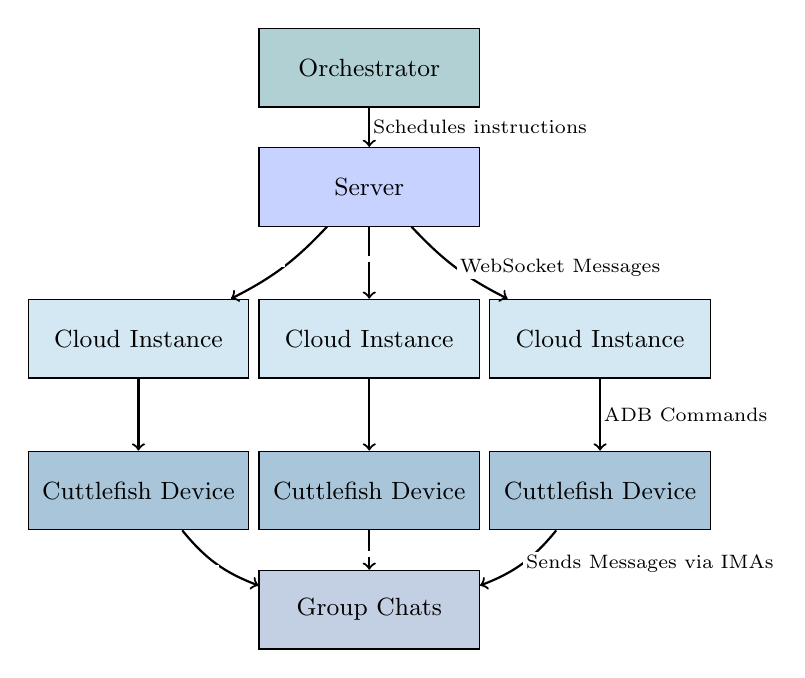
\begin{tikzpicture}[
        node distance=1.4cm and 2.2cm,
        every node/.style={font=\small},
        block/.style={rectangle, draw, minimum width=2.8cm, minimum height=1cm, align=center},
        layer/.style={rectangle, draw=none, minimum height=0.5cm},
        line/.style={->, thick},
        textnode/.style={font=\scriptsize, midway, fill=white, inner sep=1pt}
    ]

        % Server
        \node[block, fill=pastelblue1] (orchestrator) {Orchestrator};
        \node[block, fill=pastelblue2, below=0.5cm of orchestrator] (server) {Server};

        % Clients
        \node[layer, below=0.3cm of server] (clientslabel) {};
        \node[block, fill=pastelblue3, below left=0.1cm and 1.4cm of clientslabel] (instance1) {Cloud Instance};
        \node[block, fill=pastelblue3, below=0.1cm of clientslabel] (instance2) {Cloud Instance};
        \node[block, fill=pastelblue3, below right=0.1cm and 1.4cm of clientslabel] (instance3) {Cloud Instance};

        % Traffic Capture
        \node[layer, below=0.3cm of instance2] (trafficlabel) {};
        \node[block, fill=pastelblue4, below left=0.1cm and 1.4cm of trafficlabel] (device1) {Cuttlefish Device};
        \node[block, fill=pastelblue4, below=0.1cm of trafficlabel] (device2) {Cuttlefish Device};
        \node[block, fill=pastelblue4, below right=0.1cm and 1.4cm of trafficlabel] (device3) {Cuttlefish Device};

        % Group Chats
        \node[block, fill=pastelblue5, below=0.5cm of device2] (groupchats) {Group Chats};

        % Arrows from Orchestrator to Server
        \draw[line] (orchestrator) -- node[textnode, right] {Schedules instructions} (server);

        % Arrows from Orchestrator to Instances
        \draw[line] (server) to[bend left=10] node[textnode, above] {} (instance1);
        \draw[line] (server) -- node[textnode, above] {} (instance2);
        \draw[line] (server) to[bend right=10] node[textnode, right] {WebSocket Messages} (instance3);

        % ADB Commands from Instances to Devices
        \draw[line] (instance1) -- node[textnode, left] {} (device1);
        \draw[line] (instance2) -- node[textnode, left] {} (device2);
        \draw[line] (instance3) -- node[textnode, right] {ADB Commands} (device3);

        % IMAs arrows to Group Chats
        \draw[line] (device1) to[bend right=15] node[textnode, below] {} (groupchats);
        \draw[line] (device2) -- node[textnode, below] {} (groupchats);
        \draw[line] (device3) to[bend left=15] node[textnode, right] {Sends Messages via IMAs} (groupchats);

    \end{tikzpicture}
    \DIFaddendFL \caption{Experiment architecture overview}
    \label{fig:architecture}
\end{figure}
\DIFdelbegin %DIFDELCMD < 

%DIFDELCMD < %%%
\DIFdel{Figure \ref{fig:architecture} illustrates the }\DIFdelend \DIFaddbegin \DIFadd{The }\DIFaddend end-to-end architecture for generating encrypted group chat traffic \DIFaddbegin \DIFadd{is illustrated in Figure \ref{fig:architecture}}\DIFaddend . Our system \DIFdelbegin \DIFdel{leverages }\DIFdelend \DIFaddbegin \DIFadd{utilizes }\DIFaddend three Google Cloud instances running Ubuntu 20.04 LTS to emulate Android smartphones \DIFdelbegin \DIFdel{via }\DIFdelend \DIFaddbegin \DIFadd{using }\DIFaddend Android Cuttlefish\footnote{Each instance is provisioned with 2 vCPUs, 13 GB RAM, and 400 GB SSD storage.}. These \DIFdelbegin \DIFdel{instances host 8 popular IMAsto simulate multi-device group interactions}\DIFdelend \DIFaddbegin \DIFadd{Cuttlefish instances host eight IMAs}\DIFaddend .

\DIFdelbegin \DIFdel{A Python-based orchestration framework coordinates message delivery }\DIFdelend \DIFaddbegin \DIFadd{An orchestration framework governs message delivery across the emulated environment. On each emulated device (client), Operating System level commands, such as sending messages or switching applications, are executed via the ADB}\DIFaddend . \DIFdelbegin \DIFdel{Clients execute OS-level commands (e.g., sending messages, switching apps) via Android Debug Bridge (ADB). Server }\DIFdelend \DIFaddbegin \DIFadd{A server }\DIFaddend manages message timing and IMA selection\DIFdelbegin \DIFdel{, synchronizing conversations across }\DIFdelend \DIFaddbegin \DIFadd{. This server also synchronizes conversations across all }\DIFaddend devices through WebSocket connections.

We \DIFaddbegin \DIFadd{use tcpdump to }\DIFaddend capture encrypted traffic\DIFdelbegin \DIFdel{using tcpdump, which generates }\DIFdelend \DIFaddbegin \DIFadd{, producing }\DIFaddend PCAP files for \DIFdelbegin \DIFdel{downstream analysis. This }\DIFdelend \DIFaddbegin \DIFadd{later analysis. Our system's }\DIFaddend cloud-native \DIFdelbegin \DIFdel{design enables horizontal scalability. Additional devices can be provisioned }\DIFdelend \DIFaddbegin \DIFadd{architecture inherently supports horizontal scalability, allowing for the }\DIFaddend on-demand \DIFaddbegin \DIFadd{provisioning of additional devices }\DIFaddend to simulate larger groups\DIFdelbegin \DIFdel{without }\DIFdelend \DIFaddbegin \DIFadd{, thereby eliminating }\DIFaddend hardware dependencies.
\DIFdelbegin \DIFdel{These devices seamlessly connect to the server, thereby serving as one of our key contributions to IMA data generation. }\DIFdelend 

\DIFaddbegin \DIFadd{For the purpose of this study, asynchronous chat is defined as a multi-user interaction. Such interactions are characterized by irregular, delayed replies that do not adhere to strict timing or sequencing. }\DIFaddend To replicate the \DIFdelbegin \DIFdel{organic }\DIFdelend dynamics of real-world group chats, our framework generates \DIFdelbegin \DIFdel{conversations that }\DIFdelend \DIFaddbegin \DIFadd{asynchronous conversations. These conversations are designed to }\DIFaddend mirror human behavior across \DIFaddbegin \DIFadd{various }\DIFaddend devices and IMAs.
\DIFdelbegin \DIFdel{We define asynchronous chat as a multi-user interaction with irregular, delayed replies lacking strict timing or sequencing. Using publicly available data sources }\DIFdelend \DIFaddbegin 

\DIFadd{The system leverages publicly available datasets }\DIFaddend of natural dialogue\DIFdelbegin \DIFdel{, the system assigns lines to devices and applications (e.g., Slack, Signal) with }\DIFdelend \DIFaddbegin \DIFadd{. From these datasets, it assigns dialogue lines to specific devices and IMAs. This process incorporates }\DIFaddend randomized wait times\DIFdelbegin \DIFdel{(}\DIFdelend \DIFaddbegin \DIFadd{, ranging from }\DIFaddend 15 \DIFdelbegin \DIFdel{–}\DIFdelend \DIFaddbegin \DIFadd{to }\DIFaddend 60 seconds\DIFdelbegin \DIFdel{) shown }\DIFdelend \DIFaddbegin \DIFadd{, as detailed }\DIFaddend in Table \ref{tab:Top5TrimmedDialogue}\DIFdelbegin \DIFdel{, mimicking }\DIFdelend \DIFaddbegin \DIFadd{. This randomization effectively mimics }\DIFaddend the irregular pacing of actual conversations\DIFdelbegin \DIFdel{—}\DIFdelend \DIFaddbegin \DIFadd{. For instance, it accommodates }\DIFaddend longer pauses for complex replies \DIFdelbegin \DIFdel{, shorter gaps for }\DIFdelend \DIFaddbegin \DIFadd{and allows for shorter gaps during }\DIFaddend quick responses. \DIFdelbegin \DIFdel{Messages }\DIFdelend \DIFaddbegin \DIFadd{To further emulate the brevity of mobile chats, messages }\DIFaddend are limited to \DIFaddbegin \DIFadd{the }\DIFaddend first 50 characters\DIFaddbegin \DIFadd{.
Furthermore, the framework captures the multi-platform spontaneity inherent in real group interactions. It achieves this by distributing dialogues across multiple IMAs; for example}\DIFaddend , \DIFdelbegin \DIFdel{emulating the brevity of mobile chats. By distributing dialogues to multiple IMAs(e.g., }\DIFdelend a debate \DIFdelbegin \DIFdel{starting }\DIFdelend \DIFaddbegin \DIFadd{might initiate }\DIFaddend in Teams and \DIFdelbegin \DIFdel{continuing in Telegram), the framework captures the multi-platform spontaneity of real group interactions.
While this work }\DIFdelend \DIFaddbegin \DIFadd{subsequently continue in Telegram.
}

\DIFadd{Although the current study }\DIFaddend focuses on general chat activity \DIFdelbegin \DIFdel{sufficient }\DIFdelend \DIFaddbegin \DIFadd{adequate }\DIFaddend for IMA identification, future iterations \DIFdelbegin \DIFdel{aimed at feature-level identification would require }\DIFdelend \DIFaddbegin \DIFadd{will need to address a broader scope. Specifically, they will necessitate }\DIFaddend generating traffic associated with distinct actions \DIFdelbegin \DIFdel{like }\DIFdelend \DIFaddbegin \DIFadd{within each IMA, such as }\DIFaddend voice call initiation, file uploading, or video streaming\DIFdelbegin \DIFdel{within each IMA}\DIFdelend .

\begin{table}[!ht]
\centering
\caption{dialogue schedule snippet}
\label{tab:Top5TrimmedDialogue}
\resizebox{0.9\columnwidth}{!}{%
\begin{tabular}{|l|c|c|c|}
\hline
\multicolumn{1}{|c|}{\textbf{Dialogue}} & \textbf{Device} & \textbf{IMA} & \textbf{Wait Time (seconds)} \\ \hline
Nay, answer me. ...                      & 3              & signal       & 45                          \\ \hline
He. ...                                  & 2              & signal       & 60                          \\ \hline
You come most ...                        & 3              & teams        & 55                          \\ \hline
Not a mouse ...                          & 3              & skype        & 58                          \\ \hline
Well, good night. ...                    & 1              & signal       & 33                          \\ \hline
\multicolumn{4}{|c|}{\textit{... conversation continues ...}} \\ \hline
\end{tabular}%
}
\end{table}

\subsection{Traffic Orchestration and Client-Device Interaction}
\DIFdelbegin %DIFDELCMD < 

%DIFDELCMD < %%%
\DIFdel{A Python-based orchestrator}\DIFdelend \DIFaddbegin \DIFadd{An orchestrator, }\DIFaddend running on the server\DIFaddbegin \DIFadd{, }\DIFaddend manages device-specific message queues\DIFdelbegin \DIFdel{, preventing bottlenecks as it schedules messages }\DIFdelend \DIFaddbegin \DIFadd{. This management prevents bottlenecks by efficiently scheduling messages derived }\DIFaddend from the emulated dialogue data. Once the \DIFdelbegin \DIFdel{schedule is set}\DIFdelend \DIFaddbegin \DIFadd{message schedule is determined}\DIFaddend , the orchestrator \DIFaddbegin \DIFadd{performs several actions. First, it }\DIFaddend establishes a WebSocket connection\DIFdelbegin \DIFdel{, }\DIFdelend \DIFaddbegin \DIFadd{. Then, it }\DIFaddend declares the number of \DIFdelbegin \DIFdel{devices to expect, and relays messages accordingly}\DIFdelend \DIFaddbegin \DIFadd{Cuttlefish devices expected to connect. Finally, it relays messages to these devices according to the schedule}\DIFaddend . As each Cuttlefish device registers \DIFdelbegin \DIFdel{via WebSocket}\DIFdelend \DIFaddbegin \DIFadd{with the server via its WebSocket connection}\DIFaddend , the server assigns it a \DIFdelbegin \DIFdel{numeric ID and }\DIFdelend \DIFaddbegin \DIFadd{unique numeric ID. Subsequently, the server }\DIFaddend routes the appropriate messages \DIFaddbegin \DIFadd{to that specific device }\DIFaddend in real time.

On the client side, each Cuttlefish device \DIFdelbegin \DIFdel{runs a script that receives servercommands, executing them via }\DIFdelend \DIFaddbegin \DIFadd{operates under the control of a dedicated script. This script is responsible for receiving commands from the server. It then executes these commands using }\DIFaddend the Android Debug Bridge (ADB). \DIFdelbegin \DIFdel{These commands }\DIFdelend \DIFaddbegin \DIFadd{The commands issued by the server direct the Cuttlefish devices to }\DIFaddend emulate user interactions\DIFdelbegin \DIFdel{(e.g., }\DIFdelend \DIFaddbegin \DIFadd{. These interactions, such as }\DIFaddend taps, swipes, \DIFdelbegin \DIFdel{keyboard input) through }\DIFdelend \DIFaddbegin \DIFadd{and keyboard input, are performed according to }\DIFaddend predefined scripts. Consequently, each device \DIFaddbegin \DIFadd{actively }\DIFaddend sends text messages to group chats \DIFdelbegin \DIFdel{in multiple IMAs, automatically switching among apps to simulate }\DIFdelend \DIFaddbegin \DIFadd{within multiple IMAs. The devices also automatically switch among these applications, simulating }\DIFaddend realistic multi-application \DIFdelbegin \DIFdel{behavior. 
This integrated design allows us to capture concurrent traffic flows from multiple IMAs and devices in a synchronized manner.
}\DIFdelend \DIFaddbegin \DIFadd{usage patterns. 
}\DIFaddend 

\subsection{Traffic Capture and Labeling}
\DIFdelbegin \DIFdel{Encrypted }\DIFdelend \DIFaddbegin \DIFadd{First, encrypted }\DIFaddend traffic is captured using \DIFaddbegin \DIFadd{the }\DIFaddend \texttt{tcpdump} \DIFdelbegin \DIFdel{and isolatedthrough dynamic filters}\DIFdelend \DIFaddbegin \DIFadd{utility. This captured traffic is subsequently isolated. The isolation process utilizes dynamic filters, which are }\DIFaddend generated from \texttt{netstat} logs\DIFaddbegin \DIFadd{. These }\texttt{\DIFadd{netstat}} \DIFadd{logs are }\DIFaddend collected at 60-second intervals. \DIFdelbegin \DIFdel{These logs are processed }\DIFdelend \DIFaddbegin \DIFadd{Next, these logs undergo processing. They are transformed }\DIFaddend into a JSON-structured session database\DIFdelbegin \DIFdel{recording IMA-specific }\DIFdelend \DIFaddbegin \DIFadd{. This database records specific details for each IMA, including associated }\DIFaddend ports, IP addresses, and \DIFdelbegin \DIFdel{timestamps (e.g., }\DIFdelend \DIFaddbegin \DIFadd{activity timestamps. For example, an entry might indicate }\DIFaddend port \texttt{51558} \DIFaddbegin \DIFadd{was }\DIFaddend active between UNIX epochs \texttt{\DIFdelbegin \DIFdel{1726056090--1726057619}%DIFDELCMD < \MBLOCKRIGHTBRACE%%%
\DIFdel{). The }\DIFdelend \DIFaddbegin \DIFadd{1726056090 and 1726057619}}\DIFadd{. To achieve precise traffic isolation, the }\DIFaddend following methodologies are then applied:

\begin{itemize}
    \item \textbf{Time-Bounded Port/IP Correlation}: Matches active ports/IPs from \texttt{netstat} logs (e.g., \texttt{192.168.97.2:59895 → 52.157.5.65:443}) with \DIFdelbegin \DIFdel{precise timestamps to create }\DIFdelend \DIFaddbegin \DIFadd{timestamps for }\DIFaddend session-aware filters \DIFdelbegin \DIFdel{. For example, a }\DIFdelend \DIFaddbegin \DIFadd{(e.g., }\DIFaddend Teams call on port \texttt{51558} \DIFdelbegin \DIFdel{would only be isolated during its recorded active windows.
    }%DIFDELCMD < 

%DIFDELCMD <     %%%
\DIFdelend \DIFaddbegin \DIFadd{isolated during active windows).
    }\DIFaddend \item \textbf{TLS SNI Disambiguation}: Resolves port conflicts (e.g., Slack/WhatsApp on 443) by extracting SNI fields from TLS ClientHello packets (e.g., \texttt{*.signal.org} for Signal).
    \DIFdelbegin %DIFDELCMD < 

%DIFDELCMD <     %%%
\DIFdelend \item \textbf{Application-Aware IP Whitelisting}: Identifies IMAs using known static IP ranges (e.g., Telegram's \texttt{51.81.11.66}), bypassing ephemeral port limitations.
\end{itemize}

\begin{lstlisting}[
    language=,  % Remove "json" - this is Wireshark filter syntax
    basicstyle=\ttfamily\footnotesize,
    breaklines=true,
    caption={Hypothetical Hybrid Wireshark filter combining time windows, IP whitelisting, and SNI validation for Discord.},
    label={lst:wireshark}
]
((tcp.port == 51558 AND  // Discord sessions
   frame.time_epoch >= 1726056090 AND 
   frame.time_epoch <= 1726057619) OR
  (tcp.port == 51558 AND 
   frame.time_epoch >= 1726126204 AND 
   frame.time_epoch <= 1726127414) OR
  (ip.addr == 51.81.11.66 OR ip.addr == 51.81.47.120) OR  // Discord IP ranges
  (tls.handshake.extensions_server_name contains "discord.org"))  // Discord SNI
\end{lstlisting}

\textbf{Filter Breakdown in Listing \ref{lst:wireshark}:}
\begin{itemize}
    \item Lines 1-4: Isolates Discord traffic on port \texttt{51558} during two recorded session windows.
    \item Line 5: Tags Discord traffic using its known IP addresses recorded.
    \item Lines \DIFdelbegin \DIFdel{6-}\DIFdelend \DIFaddbegin \DIFadd{6 onwards}\DIFaddend : Validates Discord traffic via SNI fields, resolving HTTPS/443 ambiguity.
\end{itemize}

After isolation of traffic, traffic flows are extracted using Tranalyzer2 \footnote{https://tranalyzer.com/} before labeling network traffic with the corresponding IMA. Tranalyzer2 determines 109 features, representing a broad range of traffic characteristics\DIFdelbegin \DIFdel{; this comprehensive set was chosen as a starting point for feature selection to ensure potential distinguishing patterns were captured}\DIFdelend .

\subsection{Apps and Device Multi-classification}
To identify both the IMAs and the source device, we first performed feature selection on the 109 extracted traffic attributes. Techniques such as mutual information and the ANOVA F-value were used to filter out the most relevant features, while hierarchical clustering with dendrograms helped reduce dimensionality.

Next, we applied a multi-output approach, allowing simultaneous prediction of the IMA label and the originating device. We \DIFdelbegin \DIFdel{utilized both }\DIFdelend \DIFaddbegin \DIFadd{used }\DIFaddend scikit-learn\footnote{https://scikit-learn.org} \DIFdelbegin \DIFdel{and cuML}\footnote{\DIFdel{https://rapids.ai/}} %DIFAUXCMD
\addtocounter{footnote}{-1}%DIFAUXCMD
\DIFdel{libraries, enabling GPU/CPU-based training depending on each algorithm’s computational requirements. For instance, due to prolonged CPU training times (}\DIFdelend \DIFaddbegin \DIFadd{for most of our algorithms. However, some models, like Support Vector Machines, were computationally intensive and took }\DIFaddend over 40 hours \DIFdelbegin \DIFdel{) on our dataset, we used cuML to accelerate Support Vector Machine training, while scikit-learn was employed for Decision Tree, Random Forest, Gradient Boosting and Naive Bayes}\DIFdelend \DIFaddbegin \DIFadd{to train on a CPU using our dataset. To accelerate this process, we employed the GPU-accelerated cuML}\footnote{\DIFadd{https://rapids.ai/}} \DIFadd{library for these models}\DIFaddend .

We evaluated each model\DIFdelbegin \DIFdel{’}\DIFdelend \DIFaddbegin \DIFadd{'}\DIFaddend s performance using accuracy, precision, recall, and F1-score, and further analyzed results with confusion matrices. A 10-fold cross-validation was conducted to gauge the models\DIFdelbegin \DIFdel{’ }\DIFdelend \DIFaddbegin \DIFadd{' }\DIFaddend consistency, capturing both average performance and potential worst-case scenarios.

\subsection{Distinguishing the User Actions (Group vs. 1:1 Chat)}
\DIFdelbegin \DIFdel{To validate if distinct communication types can be distinguished for granular NIM policies based on their intrinsic patterns, we }\DIFdelend \DIFaddbegin \DIFadd{We }\DIFaddend conducted a binary classification experiment \DIFdelbegin \DIFdel{differentiating group vs. }\DIFdelend \DIFaddbegin \DIFadd{to differentiate between group chats and }\DIFaddend 1:1 chats. \DIFaddbegin \DIFadd{The goal was to see if intrinsic traffic patterns could distinguish these communication types, which is important for creating granular NIM policies. }\DIFaddend We used a combined dataset comprising direct messaging traffic data from Erdenebaatar et al.\cite{b1} and the group chat traffic data we generated (Section III-B/C) aiding the model in identifying fundamental structural differences.

Our feature engineering focused \DIFdelbegin \DIFdel{explicitly }\DIFdelend on distilling core communication patterns thought to be inherent to the interaction type, rather than the network environment. We calculated relational ratios (e.g., sent/received bytes/packets) reflecting conversational balance, used normalized timing features (e.g., inter-arrival times) to capture relative pacing, and developed structural indicators of message flow, independent of absolute network speeds or latencies. Conversely, we excluded low-level TCP metrics (e.g., \DIFdelbegin \DIFdel{tcpSeqSntBytes, tcpWinSzChgDirCnt) potentially dominated }\DIFdelend \DIFaddbegin \DIFadd{`tcpSeqSntBytes`, `tcpWinSzChgDirCnt`). We did this because these metrics are often heavily influenced }\DIFaddend by network conditions rather than the communication pattern itself\DIFdelbegin \DIFdel{, as these }\DIFdelend \DIFaddbegin \DIFadd{. Therefore, they }\DIFaddend would be less reliable for a practical NIM system \DIFdelbegin \DIFdel{operating }\DIFdelend \DIFaddbegin \DIFadd{that needs to operate }\DIFaddend across varied environments.

We evaluated several ML algorithms for classification, including those used for application/device identification (Section III-F). Gradient Boosting provided the best performance in differentiating group vs. 1:1 chats based on these distilled patterns. Structured cross-validation and dimensionality reduction were used throughout the evaluation to confirm that classification relied on meaningful behavioral patterns, suitable for reliable NIM decisions.

\section{Evaluation and Results}
\DIFdelbegin %DIFDELCMD < 

%DIFDELCMD < %%%
\DIFdelend \subsection{Dataset and Traffic Characteristics}
\DIFdelbegin %DIFDELCMD < 

%DIFDELCMD < %%%
\DIFdelend As demonstrated by our results, this scalable approach successfully produced 37 hours of encrypted group chat traffic that closely mirrors real-device performance—even across eight IMAs\DIFdelbegin \DIFdel{—}\DIFdelend \DIFaddbegin \DIFadd{, }\DIFaddend with consistent flow characteristics and sufficient variability to train our ML models. As shown in Table \ref{tab:flowExtraction}, Slack had the highest data volume (36.33 MB per device) and Teams produced the most flows (4,052 on Device 1). Device 1 consistently generated 15–20\% more traffic than Devices 2/3, likely due to the randomized emulated conversations (Section III-C).


\subsection{Feature Selection and Impact}
\DIFdelbegin %DIFDELCMD < 

%DIFDELCMD < %%%
\DIFdelend ANOVA F-value analysis (Table \ref{tab:TP}) identified critical features for distinguishing IMAs without decrypting messages: \begin{enumerate} 
    \item \textbf{tcpMSS}: Differentiates Discord and Slack. 
    \item \textbf{ipMaxdIPID}: Flags Signal, Skype, and Telegram. 
    \item \textbf{tcpMinWinSz}: Highlights bulk transfers in Skype and Teams. 
\end{enumerate} 
These features are fundamental to our ML framework, directly enabling both application and device-level identification and \DIFdelbegin \DIFdel{supporting our ability to trace }\DIFdelend \DIFaddbegin \DIFadd{providing foundational support for tasks such as tracing }\DIFaddend malicious activity.

\begin{table}[!ht]
\centering
\caption{IMA Anova F-Value Top 5 Features}
\label{tab:TP}
\resizebox{\columnwidth}{!}{%
\begin{tabular}{|l|c|c|c|}
\hline
\multicolumn{1}{|c|}{\textbf{Rank}} & \textbf{Feature} & \textbf{\begin{tabular}[c]{@{}c@{}}Normalized \\ F-Score\end{tabular}} & \textbf{Description} \\ \hline
1 & tcpMSS & 1.000 & \begin{tabular}[c]{@{}c@{}}Max bytes in a single TCP segment.\end{tabular} \\ \hline
2 & ipMaxdIPID & 0.578 & \begin{tabular}[c]{@{}c@{}}Max IP ID delta between packets.\end{tabular} \\ \hline
3 & ipMinTTL & 0.576 & \begin{tabular}[c]{@{}c@{}}Minimum TTL observed in IP packets.\end{tabular} \\ \hline
4 & dstPort & 0.569 & \begin{tabular}[c]{@{}c@{}}Destination port number.\end{tabular} \\ \hline
5 & tcpMinWinSz & 0.568 & \begin{tabular}[c]{@{}c@{}}Smallest TCP window size.\end{tabular} \\ \hline
\end{tabular}%
}
\end{table}

\begin{table}[!ht]
\centering
\caption{IMA flow extraction information}
\label{tab:flowExtraction}
\resizebox{\columnwidth}{!}{%
\begin{tabular}{|l|l|c|c|c|}
\hline
                              & \multicolumn{1}{c|}{\textbf{IMA}} & \textbf{\# of Packets} & \textbf{Total Size (Mb)} & \textbf{Total \# of Flows} \\ \hline
\multirow{8}{*}{Device 1} & Discord                           & 24878                 & 10                       & 612                        \\ \cline{2-5} 
                              & Messenger                         & 39891                 & 12                       & 1556                       \\ \cline{2-5} 
                              & RocketChat                        & 33680                 & 5                        & 499                        \\ \cline{2-5} 
                              & Slack                             & 107303                & 36                       & 1838                       \\ \cline{2-5} 
                              & Skype                             & 43825                 & 28                       & 2261                       \\ \cline{2-5} 
                              & Signal                            & 54699                 & 10                       & 704                        \\ \cline{2-5} 
                              & Teams                             & 70473                 & 37                       & 4052                       \\ \cline{2-5} 
                              & Telegram                          & 23690                 & 5                        & 866                        \\ \hline
\multirow{8}{*}{Device 2} & Discord                           & 24767                 & 7                        & 631                        \\ \cline{2-5} 
                              & Messenger                         & 42945                 & 13                       & 1589                       \\ \cline{2-5} 
                              & RocketChat                        & 32583                 & 5                        & 406                        \\ \cline{2-5} 
                              & Slack                             & 113898                & 38                       & 1809                       \\ \cline{2-5} 
                              & Skype                             & 37218                 & 24                       & 1774                       \\ \cline{2-5} 
                              & Signal                            & 52069                 & 10                       & 824                        \\ \cline{2-5} 
                              & Teams                             & 59543                 & 31                       & 3448                       \\ \cline{2-5} 
                              & Telegram                          & 22958                 & 4                        & 812                        \\ \hline
\multirow{8}{*}{Device 3} & Discord                           & 23586                 & 6                        & 596                        \\ \cline{2-5} 
                              & Messenger                         & 34949                 & 11                       & 1477                       \\ \cline{2-5} 
                              & RocketChat                        & 35241                 & 5                        & 431                        \\ \cline{2-5} 
                              & Slack                             & 107275                & 35                       & 1791                       \\ \cline{2-5} 
                              & Skype                             & 32635                 & 22                       & 1673                       \\ \cline{2-5} 
                              & Signal                            & 53627                 & 10                       & 696                        \\ \cline{2-5} 
                              & Teams                             & 52754                 & 27                       & 3163                       \\ \cline{2-5} 
                              & Telegram                          & 23791                 & 4                        & 797                        \\ \hline
\end{tabular}%
}
\end{table}

\subsection{\DIFdelbegin \DIFdel{Key Performance Indicators}\DIFdelend \DIFaddbegin \DIFadd{Measuring Success}\DIFaddend }
\DIFdelbegin %DIFDELCMD < 

%DIFDELCMD < %%%
\DIFdelend Tree-based methods (Decision Tree, Random Forest, Gradient Boosting) excel on the 109-feature dataset \DIFdelbegin \DIFdel{(Table \ref{tab:MLDevresults}}\DIFdelend \DIFaddbegin \DIFadd{for IMA classification (Table \ref{tab:MinMaxeresults}}\DIFaddend ). In particular, the Gradient Boosting model achieved an F1-score exceeding 97\%.
%DIF < while Logistic Regression achieved around 94\%, and both Naive Bayes and SVM underperformed by comparison. 
\DIFdelbegin \DIFdel{Figure \ref{fig:example} illustrates a typical Gradient Boosting confusion matrix where most misclassifications are attributed to endpoint overlaps in Microsoft’s infrastructure or inherent model limitations.
}\DIFdelend 

As demonstrated by our experimental results, our ML framework achieved a 98.6\% F1-score in distinguishing between eight IMAs, thereby confirming our goal of high-precision identification in complex, multi-user environments. A 10-fold cross-validation yielded a 98.6\% F1-score, and testing on a 20\% holdout subset achieved 97.8\%, \DIFdelbegin \DIFdel{thereby }\DIFdelend confirming the robustness of our approach.

\begin{table*}[!ht]
\centering
\caption{Min-Max results}
\label{tab:MinMaxeresults} 
%\resizebox{\textwidth}{!}{%
\DIFdelbeginFL %DIFDELCMD < \resizebox{15cm}{!}{%
%DIFDELCMD < \begin{tabular}{|l|ccc|ccc|ccc|}
%DIFDELCMD < \hline
%DIFDELCMD < \multicolumn{1}{|c|}{\multirow{2}{*}{\textbf{Model}}}            & \multicolumn{3}{c|}{\textbf{\begin{tabular}[c]{@{}c@{}}IMA Application\\ Classification\end{tabular}}}                                                                                                                                              & \multicolumn{3}{c|}{\textbf{Device Identification}}                                                                                                                                                                                              & \multicolumn{3}{c|}{\textbf{\begin{tabular}[c]{@{}c@{}}Group vs 1.1 user action\\ Classification\end{tabular}}}                                                                                                                      \\ \cline{2-10} 
%DIFDELCMD < \multicolumn{1}{|c|}{}                                           & \multicolumn{1}{l|}{\textit{Precision}}                                                & \multicolumn{1}{l|}{\textit{Recall}}                                                   & \multicolumn{1}{l|}{\textit{F1-Score}}                            & \multicolumn{1}{l|}{\textit{Precision}}                                               & \multicolumn{1}{l|}{\textit{Recall}}                                                  & \multicolumn{1}{l|}{\textit{F1-Score}}                           & \multicolumn{1}{l|}{\textit{Precision}}                                              & \multicolumn{1}{l|}{\textit{Recall}}                                        & \multicolumn{1}{l|}{\textit{F1-Score}}                          \\ \hline
%DIFDELCMD < \begin{tabular}[c]{@{}l@{}}Naive \\ Bayes\end{tabular}           & \multicolumn{1}{c|}{\begin{tabular}[c]{@{}c@{}}0.673 -\\  0.715\end{tabular}}          & \multicolumn{1}{c|}{\begin{tabular}[c]{@{}c@{}}0.720 - \\ 0.762\end{tabular}}          & \begin{tabular}[c]{@{}c@{}}0.647 - \\ 0.700\end{tabular}          & \multicolumn{1}{c|}{\begin{tabular}[c]{@{}c@{}}0.2304 - \\ 0.4321\end{tabular}}       & \multicolumn{1}{c|}{\begin{tabular}[c]{@{}c@{}}0.3335 - \\ 0.3596\end{tabular}}       & \begin{tabular}[c]{@{}c@{}}0.1998 - \\ 0.2656\end{tabular}       & \multicolumn{1}{c|}{\begin{tabular}[c]{@{}c@{}}0.254-\\ 0.888\end{tabular}}          & \multicolumn{1}{c|}{\begin{tabular}[c]{@{}c@{}}0.369-\\ 0.89\end{tabular}}  & \begin{tabular}[c]{@{}c@{}}0.301-\\ 0.889\end{tabular}          \\ \hline
%DIFDELCMD < \begin{tabular}[c]{@{}l@{}}Decision \\ Tree\end{tabular}         & \multicolumn{1}{c|}{\begin{tabular}[c]{@{}c@{}}0.964 -\\  0.975\end{tabular}}          & \multicolumn{1}{c|}{\begin{tabular}[c]{@{}c@{}}0.964 -\\  0.977\end{tabular}}          & \begin{tabular}[c]{@{}c@{}}0.965 -\\  0.975\end{tabular}          & \multicolumn{1}{c|}{\begin{tabular}[c]{@{}c@{}}0.9994 - \\ 1.0\end{tabular}}          & \multicolumn{1}{c|}{\begin{tabular}[c]{@{}c@{}}0.9994 -\\ 1.0\end{tabular}}           & \begin{tabular}[c]{@{}c@{}}0.9994 - \\ 1.0\end{tabular}          & \multicolumn{1}{c|}{\begin{tabular}[c]{@{}c@{}}0.274-\\ 0.878\end{tabular}}          & \multicolumn{1}{c|}{\begin{tabular}[c]{@{}c@{}}0.43-\\ 0.874\end{tabular}}  & \begin{tabular}[c]{@{}c@{}}0.335-\\ 0.876\end{tabular}          \\ \hline
%DIFDELCMD < \begin{tabular}[c]{@{}l@{}}Random \\ Forest\end{tabular}         & \multicolumn{1}{c|}{\begin{tabular}[c]{@{}c@{}}0.968 - \\ 0.977\end{tabular}}          & \multicolumn{1}{c|}{\begin{tabular}[c]{@{}c@{}}0.967 - \\ 0.977\end{tabular}}          & \begin{tabular}[c]{@{}c@{}}0.967 - \\ 0.977\end{tabular}          & \multicolumn{1}{c|}{\begin{tabular}[c]{@{}c@{}}0.9951 - \\ 0.9973\end{tabular}}       & \multicolumn{1}{c|}{\begin{tabular}[c]{@{}c@{}}0.9949 -\\  0.9974\end{tabular}}       & \begin{tabular}[c]{@{}c@{}}0.9950 - \\ 0.9973\end{tabular}       & \multicolumn{1}{c|}{\begin{tabular}[c]{@{}c@{}}0.266-\\ 0.905\end{tabular}}          & \multicolumn{1}{c|}{\begin{tabular}[c]{@{}c@{}}0.404-\\ 0.894\end{tabular}} & \begin{tabular}[c]{@{}c@{}}0.321-\\ 0.898\end{tabular}          \\ \hline
%DIFDELCMD < \begin{tabular}[c]{@{}l@{}}Gradient\\ Boosting\end{tabular}      & \multicolumn{1}{c|}{\textbf{\begin{tabular}[c]{@{}c@{}}0.977 - \\ 0.986\end{tabular}}} & \multicolumn{1}{c|}{\textbf{\begin{tabular}[c]{@{}c@{}}0.976 - \\ 0.985\end{tabular}}} & \textbf{\begin{tabular}[c]{@{}c@{}}0.976 - \\ 0.986\end{tabular}} & \multicolumn{1}{c|}{\textbf{\begin{tabular}[c]{@{}c@{}}0.9997 - \\ 1.0\end{tabular}}} & \multicolumn{1}{c|}{\textbf{\begin{tabular}[c]{@{}c@{}}0.9997 - \\ 1.0\end{tabular}}} & \textbf{\begin{tabular}[c]{@{}c@{}}0.9997 - \\ 1.0\end{tabular}} & \multicolumn{1}{c|}{\begin{tabular}[c]{@{}c@{}}0.275-\\ 0.909\end{tabular}} & \multicolumn{1}{c|}{\begin{tabular}[c]{@{}c@{}}0.435-\\ 0.903\end{tabular}} & \begin{tabular}[c]{@{}c@{}}0.337-\\ 0.905\end{tabular}          \\ \hline
%DIFDELCMD < %\begin{tabular}[c]{@{}l@{}}Logistic\\ Regression\end{tabular}    & \multicolumn{1}{c|}{\begin{tabular}[c]{@{}c@{}}0.935 - \\ 0.950\end{tabular}}          & \multicolumn{1}{c|}{\begin{tabular}[c]{@{}c@{}}0.945 -\\  0.960\end{tabular}}          & \begin{tabular}[c]{@{}c@{}}0.939 - \\ 0.954\end{tabular}          & \multicolumn{1}{c|}{\begin{tabular}[c]{@{}c@{}}0.4065 - \\ 0.4304\end{tabular}}       & \multicolumn{1}{c|}{\begin{tabular}[c]{@{}c@{}}0.4112 - \\ 0.4349\end{tabular}}       & \begin{tabular}[c]{@{}c@{}}0.4071 - \\ 0.4299\end{tabular}       & \multicolumn{1}{c|}{\begin{tabular}[c]{@{}c@{}}0.636-\\ 0.991\end{tabular}}          & \multicolumn{1}{c|}{\begin{tabular}[c]{@{}c@{}}0.615-\\ 0.992\end{tabular}} & \textbf{\begin{tabular}[c]{@{}c@{}}0.609-\\ 0.992\end{tabular}} \\ \hline
%DIFDELCMD < \begin{tabular}[c]{@{}l@{}}Support Vector\\ Machine\end{tabular} & \multicolumn{1}{c|}{\begin{tabular}[c]{@{}c@{}}0.695 - \\ 0.744\end{tabular}}          & \multicolumn{1}{c|}{\begin{tabular}[c]{@{}c@{}}0.750 -\\  0.768\end{tabular}}          & \begin{tabular}[c]{@{}c@{}}0.701 - \\ 0.729\end{tabular}          & \multicolumn{1}{c|}{\begin{tabular}[c]{@{}c@{}}0.2987 - \\ 0.3301\end{tabular}}       & \multicolumn{1}{c|}{\begin{tabular}[c]{@{}c@{}}0.3110 - \\ 0.3281\end{tabular}}       & \begin{tabular}[c]{@{}c@{}}0.2317 - \\ 0.2672\end{tabular}       & \multicolumn{1}{c|}{\begin{tabular}[c]{@{}c@{}}0.257-\\ 0.914\end{tabular}}          & \multicolumn{1}{c|}{\begin{tabular}[c]{@{}c@{}}0.376-\\ 0.917\end{tabular}} & \begin{tabular}[c]{@{}c@{}}0.305-\\ 0.915\end{tabular}          \\ \hline
%DIFDELCMD < \end{tabular}%
%DIFDELCMD < }
%DIFDELCMD < %%%
\DIFdelendFL \DIFaddbeginFL \resizebox{15cm}{!}{%
\begin{tabular}{|l|ccc|ccc|ccc|}
\hline
\multicolumn{1}{|c|}{\multirow{2}{*}{\textbf{Model}}}            & \multicolumn{3}{c|}{\textbf{\begin{tabular}[c]{@{}c@{}}IMA Application\\ Classification\end{tabular}}}                                                                                                                                              & \multicolumn{3}{c|}{\textbf{Device Identification}}                                                                                                                                                                                              & \multicolumn{3}{c|}{\textbf{\begin{tabular}[c]{@{}c@{}}Group vs 1:1 user action\\ Classification\end{tabular}}}                                                                                                                      \\ \cline{2-10} 
\multicolumn{1}{|c|}{}                                           & \multicolumn{1}{l|}{\textit{Precision}}                                                & \multicolumn{1}{l|}{\textit{Recall}}                                                   & \multicolumn{1}{l|}{\textit{F1-Score}}                            & \multicolumn{1}{l|}{\textit{Precision}}                                               & \multicolumn{1}{l|}{\textit{Recall}}                                                  & \multicolumn{1}{l|}{\textit{F1-Score}}                           & \multicolumn{1}{l|}{\textit{Precision}}                                              & \multicolumn{1}{l|}{\textit{Recall}}                                        & \multicolumn{1}{l|}{\textit{F1-Score}}                          \\ \hline
\begin{tabular}[c]{@{}l@{}}Naive \\ Bayes\end{tabular}           & \multicolumn{1}{c|}{\begin{tabular}[c]{@{}c@{}}0.673 -\\  0.715\end{tabular}}          & \multicolumn{1}{c|}{\begin{tabular}[c]{@{}c@{}}0.720 - \\ 0.762\end{tabular}}          & \begin{tabular}[c]{@{}c@{}}0.647 - \\ 0.700\end{tabular}          & \multicolumn{1}{c|}{\begin{tabular}[c]{@{}c@{}}0.2304 - \\ 0.4321\end{tabular}}       & \multicolumn{1}{c|}{\begin{tabular}[c]{@{}c@{}}0.3335 - \\ 0.3596\end{tabular}}       & \begin{tabular}[c]{@{}c@{}}0.1998 - \\ 0.2656\end{tabular}       & \multicolumn{1}{c|}{\begin{tabular}[c]{@{}c@{}}0.254-\\ 0.888\end{tabular}}          & \multicolumn{1}{c|}{\begin{tabular}[c]{@{}c@{}}0.369-\\ 0.89\end{tabular}}  & \begin{tabular}[c]{@{}c@{}}0.301-\\ 0.889\end{tabular}          \\ \hline
\begin{tabular}[c]{@{}l@{}}Decision \\ Tree\end{tabular}         & \multicolumn{1}{c|}{\begin{tabular}[c]{@{}c@{}}0.964 -\\  0.975\end{tabular}}          & \multicolumn{1}{c|}{\begin{tabular}[c]{@{}c@{}}0.964 -\\  0.977\end{tabular}}          & \begin{tabular}[c]{@{}c@{}}0.965 -\\  0.975\end{tabular}          & \multicolumn{1}{c|}{\begin{tabular}[c]{@{}c@{}}0.9994 - \\ 1.0\end{tabular}}          & \multicolumn{1}{c|}{\begin{tabular}[c]{@{}c@{}}0.9994 -\\ 1.0\end{tabular}}           & \begin{tabular}[c]{@{}c@{}}0.9994 - \\ 1.0\end{tabular}          & \multicolumn{1}{c|}{\begin{tabular}[c]{@{}c@{}}0.274-\\ 0.878\end{tabular}}          & \multicolumn{1}{c|}{\begin{tabular}[c]{@{}c@{}}0.43-\\ 0.874\end{tabular}}  & \begin{tabular}[c]{@{}c@{}}0.335-\\ 0.876\end{tabular}          \\ \hline
\begin{tabular}[c]{@{}l@{}}Random \\ Forest\end{tabular}         & \multicolumn{1}{c|}{\begin{tabular}[c]{@{}c@{}}0.968 - \\ 0.977\end{tabular}}          & \multicolumn{1}{c|}{\begin{tabular}[c]{@{}c@{}}0.967 - \\ 0.977\end{tabular}}          & \begin{tabular}[c]{@{}c@{}}0.967 - \\ 0.977\end{tabular}          & \multicolumn{1}{c|}{\begin{tabular}[c]{@{}c@{}}0.9951 - \\ 0.9973\end{tabular}}       & \multicolumn{1}{c|}{\begin{tabular}[c]{@{}c@{}}0.9949 -\\  0.9974\end{tabular}}       & \begin{tabular}[c]{@{}c@{}}0.9950 - \\ 0.9973\end{tabular}       & \multicolumn{1}{c|}{\begin{tabular}[c]{@{}c@{}}0.266-\\ 0.905\end{tabular}}          & \multicolumn{1}{c|}{\begin{tabular}[c]{@{}c@{}}0.404-\\ 0.894\end{tabular}} & \begin{tabular}[c]{@{}c@{}}0.321-\\ 0.898\end{tabular}          \\ \hline
\begin{tabular}[c]{@{}l@{}}Gradient\\ Boosting\end{tabular}      & \multicolumn{1}{c|}{\textbf{\begin{tabular}[c]{@{}c@{}}0.977 - \\ 0.986\end{tabular}}} & \multicolumn{1}{c|}{\textbf{\begin{tabular}[c]{@{}c@{}}0.976 - \\ 0.985\end{tabular}}} & \textbf{\begin{tabular}[c]{@{}c@{}}0.976 - \\ 0.986\end{tabular}} & \multicolumn{1}{c|}{\textbf{\begin{tabular}[c]{@{}c@{}}0.9997 - \\ 1.0\end{tabular}}} & \multicolumn{1}{c|}{\textbf{\begin{tabular}[c]{@{}c@{}}0.9997 - \\ 1.0\end{tabular}}} & \textbf{\begin{tabular}[c]{@{}c@{}}0.9997 - \\ 1.0\end{tabular}} & \multicolumn{1}{c|}{\begin{tabular}[c]{@{}c@{}}0.275-\\ 0.909\end{tabular}} & \multicolumn{1}{c|}{\begin{tabular}[c]{@{}c@{}}0.435-\\ 0.903\end{tabular}} & \begin{tabular}[c]{@{}c@{}}0.337-\\ 0.905\end{tabular}          \\ \hline
%\begin{tabular}[c]{@{}l@{}}Logistic\\ Regression\end{tabular}    & \multicolumn{1}{c|}{\begin{tabular}[c]{@{}c@{}}0.935 - \\ 0.950\end{tabular}}          & \multicolumn{1}{c|}{\begin{tabular}[c]{@{}c@{}}0.945 -\\  0.960\end{tabular}}          & \begin{tabular}[c]{@{}c@{}}0.939 - \\ 0.954\end{tabular}          & \multicolumn{1}{c|}{\begin{tabular}[c]{@{}c@{}}0.4065 - \\ 0.4304\end{tabular}}       & \multicolumn{1}{c|}{\begin{tabular}[c]{@{}c@{}}0.4112 - \\ 0.4349\end{tabular}}       & \begin{tabular}[c]{@{}c@{}}0.4071 - \\ 0.4299\end{tabular}       & \multicolumn{1}{c|}{\begin{tabular}[c]{@{}c@{}}0.636-\\ 0.991\end{tabular}}          & \multicolumn{1}{c|}{\begin{tabular}[c]{@{}c@{}}0.615-\\ 0.992\end{tabular}} & \textbf{\begin{tabular}[c]{@{}c@{}}0.609-\\ 0.992\end{tabular}} \\ \hline
\begin{tabular}[c]{@{}l@{}}Support Vector\\ Machine\end{tabular} & \multicolumn{1}{c|}{\begin{tabular}[c]{@{}c@{}}0.695 - \\ 0.744\end{tabular}}          & \multicolumn{1}{c|}{\begin{tabular}[c]{@{}c@{}}0.750 -\\  0.768\end{tabular}}          & \begin{tabular}[c]{@{}c@{}}0.701 - \\ 0.729\end{tabular}          & \multicolumn{1}{c|}{\begin{tabular}[c]{@{}c@{}}0.2987 - \\ 0.3301\end{tabular}}       & \multicolumn{1}{c|}{\begin{tabular}[c]{@{}c@{}}0.3110 - \\ 0.3281\end{tabular}}       & \begin{tabular}[c]{@{}c@{}}0.2317 - \\ 0.2672\end{tabular}       & \multicolumn{1}{c|}{\begin{tabular}[c]{@{}c@{}}0.257-\\ 0.914\end{tabular}}          & \multicolumn{1}{c|}{\begin{tabular}[c]{@{}c@{}}0.376-\\ 0.917\end{tabular}} & \begin{tabular}[c]{@{}c@{}}0.305-\\ 0.915\end{tabular}          \\ \hline
\end{tabular}%
}
\DIFaddendFL \end{table*}

 %DIF < \begin{table*}[!ht]
%DIF < \centering
%DIF < \caption{IMA application classification min-max results}
%DIF < \label{tab:MLDevresults} 
%DIF < \resizebox{\textwidth}{!}{%
%DIF < \resizebox{16cm}{!}{%
%DIF < \begin{tabular}{|l|c|c|c|c|}
%DIF < \hline
%DIF < \multicolumn{1}{|c|}{\textbf{Model}} & \textbf{Accuracy} & \textbf{Precision} & \textbf{Recall} & \textbf{F1 Score} \\ \hline
%DIF < Naive Bayes                          & 0.585 - 0.653     & 0.673 - 0.715      & 0.720 - 0.762   & 0.647 - 0.700     \\ \hline
%DIF < Decision Tree                        & 0.953 - 0.965     & 0.964 - 0.975      & 0.964 - 0.977   & 0.965 - 0.975     \\ \hline
%DIF < Random Forest                        & 0.953 - 0.963     & 0.968 - 0.977      & 0.967 - 0.977   & 0.967 - 0.977     \\ \hline
%DIF < Gradient Boosting                    & \textbf{0.968 - 0.978}     & \textbf{0.977 - 0.986}      & \textbf{0.976 - 0.985}   & \textbf{0.976 - 0.986}     \\ \hline
%DIF < Logistic Regression                  & 0.912 - 0.926     & 0.935 - 0.950      & 0.945 - 0.960   & 0.939 - 0.954     \\ \hline
%DIF < Support Vector Machine               & 0.703 - 0.730     & 0.695 - 0.744      & 0.750 - 0.768   & 0.701 - 0.729     \\ \hline
%DIF < \end{tabular}%
%DIF < }
%DIF < \end{table*}
%DIF >  HIGHLIGHT: COMMENTED OUT CONFUSION MATRIX
 %DIF >  \begin{figure}[!ht]
 %DIF >      \centering
 %DIF >      \includegraphics[width=0.45\textwidth]{Figure_2.png}
 %DIF >      \caption{Gradient Boosting application confusion matrix}
 %DIF >      \label{fig:example}
 %DIF >  \end{figure}

\DIFdelbegin %DIFDELCMD < \begin{figure}[!ht]
%DIFDELCMD <      \centering
%DIFDELCMD <      \includegraphics[width=0.45\textwidth]{Figure_2.png}
%DIFDELCMD <      %%%
%DIFDELCMD < \caption{%
{%DIFAUXCMD
\DIFdelFL{Gradient Boosting application confusion matrix}}
     %DIFAUXCMD
%DIFDELCMD < \label{fig:example}
%DIFDELCMD <  \end{figure}
%DIFDELCMD < 

%DIFDELCMD < %%%
\DIFdelend \subsection{Device Identification Results}
\DIFdelbegin %DIFDELCMD < 

%DIFDELCMD < %%%
\DIFdelend For device identification, we assigned three labels (Device1, Device2, Device3) and observed that tree-based algorithms again delivered the highest performance (Table \ref{tab:MinMaxeresults}). The Gradient Boosting model achieved near-perfect results in our 10-fold tests—with eight folds reaching 100\% F1-score and the remaining two folds above 99.9\%. These findings underscore our framework\DIFdelbegin \DIFdel{’}\DIFdelend \DIFaddbegin \DIFadd{'}\DIFaddend s ability to precisely map encrypted flows to specific devices, a critical aspect of our contribution. This precision is \DIFdelbegin \DIFdel{essential }\DIFdelend \DIFaddbegin \DIFadd{a critical prerequisite }\DIFaddend for real-world scenarios \DIFdelbegin \DIFdel{, }\DIFdelend such as tracing and isolating malicious or compromised devices in complex group chat environments, all without decrypting message contents.

%DIF < \begin{table*}[!ht]
%DIF < \centering
%DIF < \caption{Device identification min-max results}
%DIF < \label{tab:MLresults}
%DIF < \resizebox{\textwidth}{!}{%
%DIF < \resizebox{16cm}{!}{%
%DIF < \begin{tabular}{|l|c|c|c|c|}
%DIF < \hline
%DIF < \multicolumn{1}{|c|}{\textbf{Model}} & \textbf{Accuracy} & \textbf{Precision} & \textbf{Recall} & \textbf{F1 Score} \\ \hline
%DIF < Naive Bayes                          & 0.3141 - 0.3579   & 0.2304 - 0.4321    & 0.3335 - 0.3596 & 0.1998 - 0.2656   \\ \hline
%DIF < Decision Tree                        & 0.9994 - 1.0      & 0.9994 - 1.0       & 0.9994 - 1.0    & 0.9994 - 1.0      \\ \hline
%DIF < Random Forest                        & 0.9950 - 0.9974   & 0.9951 - 0.9973    & 0.9949 - 0.9974 & 0.9950 - 0.9973   \\ \hline
%DIF < Gradient Boosting                    & \textbf{0.9997 - 1.0}      & \textbf{0.9997 - 1.0}       & \textbf{0.9997 - 1.0}    & \textbf{0.9997 - 1.0}      \\ \hline
%DIF < Logistic Regression                  & 0.4093 - 0.4327   & 0.4065 - 0.4304    & 0.4112 - 0.4349 & 0.4071 - 0.4299   \\ \hline
%DIF < Support Vector Machine               & 0.3284 - 0.3503   & 0.2987 - 0.3301    & 0.3110 - 0.3281 & 0.2317 - 0.2672   \\ \hline
%DIF < \end{tabular}%
%DIF < }
%DIF < /end{table*}
\DIFdelbegin %DIFDELCMD < 

%DIFDELCMD < %%%
%DIF < \begin{table*}[!ht]
%DIF < \centering
%DIF < \caption{Group vs 1:1 user action classification min-max results}
%DIF < \label{tab:MLDevresults} 
%DIF < \resizebox{\textwidth}{!}{%
%DIF < \resizebox{16cm}{!}{%
%DIF < \begin{tabular}{|l|c|c|c|c|}
%DIF < \hline
%DIF < \multicolumn{1}{|c|}{\textbf{Model}} & \textbf{Accuracy} & \textbf{Precision} & \textbf{Recall} & \textbf{F1 Score} \\ \hline
%DIF < Naive Bayes                          & 0.431-0.89     & 0.254-0.888      & 0.369-0.89   & 0.301-0.889     \\ \hline
%DIF < Decision Tree                        & 0.503-0.877     & 0.274-0.878      & %0.43-0.874   & 0.335-0.876     \\ \hline
%DIF < Random Forest                        & 0.472-0.9     & 0.266-0.905      & 0.404-0.894   & 0.321-0.898     \\ \hline
%DIF < Gradient Boosting                    & 0.508-0.906     & 0.275-0.909      & 0.435-0.903   & 0.337-0.905     \\ \hline
%DIF < \textbf{Logistic Regression}                  & 0.631-0.992     & 0.636-0.991      & 0.615-0.992   & \textbf{0.609-0.992}     \\ \hline
%DIF < Support Vector Machine               & 0.44-0.915     & 0.257-0.914      & 0.376-0.917   & 0.305-0.915     \\ \hline
%DIF < \end{tabular}%
%DIF < }
%DIF < \end{table*}
%DIFDELCMD < 

%DIFDELCMD < %%%
\DIFdelend \begin{table*}[!ht]
\centering
\caption{Group vs 1:1 user action classification for each IMA app for \textbf{Gradient Boosting}}
\label{tab:MLDevresults} 
%\resizebox{\textwidth}{!}{%
\DIFdelbeginFL %DIFDELCMD < \resizebox{10cm}{!}{%
%DIFDELCMD < \begin{tabular}{|l|c|c|c|c|}
%DIFDELCMD < \hline
%DIFDELCMD < \multicolumn{1}{|c|}{\textbf{IMA}} & \textbf{Accuracy} & \textbf{Precision} & \textbf{Recall} & \textbf{F1 Score} \\ \hline
%DIFDELCMD < \textbf{Discord}                         & 90.6\%     & 90.8\%      & 90.2\%   & \textbf{90.4\%}     \\ \hline
%DIFDELCMD < Messenger                        & 82.2\%     & 82.4\%      & 80.5\%   & 81.1\%     \\ \hline
%DIFDELCMD < Signal                        & 50.8\%     & 27.4\%      & 43.4\%   & 33.6\%     \\ \hline
%DIFDELCMD < Slack                    & 72.4\%     & 72.3\%      & 71.8\%   & 71.9\%     \\ \hline
%DIFDELCMD < Teams                 & 75.8\%     & 75.5.1\%      & 76.7\%   & 75.5\%     \\ \hline
%DIFDELCMD < Telegram               & 85.5\%     & 86.3\%      & 84.9\%   & 85.2\%     \\ \hline
%DIFDELCMD < \end{tabular}%
%DIFDELCMD < }
%DIFDELCMD < %%%
\DIFdelendFL \DIFaddbeginFL \resizebox{10cm}{!}{%
\begin{tabular}{|l|c|c|c|c|}
\hline
\multicolumn{1}{|c|}{\textbf{IMA}} & \textbf{Accuracy} & \textbf{Precision} & \textbf{Recall} & \textbf{F1 Score} \\ \hline
\textbf{Discord}                         & 90.6\%     & 90.8\%      & 90.2\%   & \textbf{90.4\%}     \\ \hline
Messenger                        & 82.2\%     & 82.4\%      & 80.5\%   & 81.1\%     \\ \hline
Signal                        & 50.8\%     & 27.4\%      & 43.4\%   & 33.6\%     \\ \hline
Slack                    & 72.4\%     & 72.3\%      & 71.8\%   & 71.9\%     \\ \hline
Teams                 & 75.8\%     & 75.5\%      & 76.7\%   & 75.5\%     \\ \hline
Telegram               & 85.5\%     & 86.3\%      & 84.9\%   & 85.2\%     \\ \hline
\end{tabular}%
}
\DIFaddendFL \end{table*}

%DIF <  \begin{figure}[!ht]
%DIF <      \centering
%DIF <      \includegraphics[width=0.45\textwidth]{Figure_3.png}
%DIF <      \caption{Gradient Boosting device confusion matrix}
%DIF <      \label{fig:example2}
%DIF <  \end{figure}
\DIFdelbegin %DIFDELCMD < 

%DIFDELCMD < %%%
\DIFdelend \subsection{Chat Type Classification Results (Group vs. 1:1)}

In the binary classification task designed to distinguish group chats from 1:1 chats using the environment-agnostic features described in Section III-G, promising results were obtained. Gradient Boosting achieved approximately 73.3\% F1-score overall. Performance varied significantly by application when evaluated using the F1-score metric for this task: classification for Discord reached 90.4\% F1, while Signal proved more challenging at 33.6\% F1, with other tested applications averaging around 78.4\% F1. \DIFdelbegin \DIFdel{While the }\DIFdelend \DIFaddbegin \DIFadd{The }\DIFaddend overall accuracy and some individual scores \DIFdelbegin \DIFdel{are lower than the primary application/device identificationresults (which }\DIFdelend \DIFaddbegin \DIFadd{for this task were lower than our primary results for application and device identification. This difference is likely because the primary tasks }\DIFaddend benefited from a richer feature set \DIFdelbegin \DIFdel{potentially including }\DIFdelend \DIFaddbegin \DIFadd{that might have included }\DIFaddend environment-specific cues\DIFdelbegin \DIFdel{), these findings , achieved across }\DIFdelend \DIFaddbegin \DIFadd{. Nevertheless, the current findings for chat type classification were achieved using }\DIFaddend diverse datasets and \DIFdelbegin \DIFdel{with features deliberately chosen }\DIFdelend \DIFaddbegin \DIFadd{features carefully selected }\DIFaddend to minimize environmental bias\DIFdelbegin \DIFdel{, }\DIFdelend \DIFaddbegin \DIFadd{. These results }\DIFaddend provide initial evidence that \DIFaddbegin \DIFadd{encrypted traffic metadata patterns alone can differentiate }\DIFaddend distinct communication structures\DIFdelbegin \DIFdel{(like group vs. }\DIFdelend \DIFaddbegin \DIFadd{, such as group versus }\DIFaddend 1:1 \DIFdelbegin \DIFdel{interaction) can indeed be differentiated based solely on encrypted traffic metadata patterns}\DIFdelend \DIFaddbegin \DIFadd{interactions}\DIFaddend .

These high F1-scores for application and device identification demonstrate the ability to reliably establish the necessary context using encrypted flow metadata within our emulated environment. These results meet our study\DIFdelbegin \DIFdel{’}\DIFdelend \DIFaddbegin \DIFadd{'}\DIFaddend s core goal and lay the foundation for future work—accurate application and device context—for \DIFdelbegin \DIFdel{Network Identity Management (NIM ) }\DIFdelend \DIFaddbegin \DIFadd{NIM }\DIFaddend systems to make informed policy decisions. Furthermore, the ~73.3\% F1-score achieved in differentiating chat types suggests the potential for subsequently investigating finer-grained, feature-level traffic classification.


\section{Discussion}
\subsection{\DIFaddbegin \DIFadd{How }\DIFaddend NIM \DIFdelbegin \DIFdel{: Network-Level Identity-Aware Access Control}\DIFdelend \DIFaddbegin \DIFadd{Works}\DIFaddend }
The core capability demonstrated in this paper—accurate identification of application and originating device from encrypted flows—is a crucial enabler for \DIFdelbegin \DIFdel{Network Identity Management (NIM).
This represents a paradigm shift towards implementing identity-aware access control directly at the network layer, even for encrypted applications.
}\DIFdelend \DIFaddbegin \DIFadd{NIM.
}\DIFaddend 

In a NIM deployment, organizations would define access groups based on roles (e.g., Developers, Executives, Contractors) and assign application permissions accordingly (e.g., Developers group allowed to have a group chat on Slack and Teams; Contractors group denied access to internal code repositories). When a device connects to the network, its traffic is associated with a verified user identity and their corresponding group memberships.

\DIFaddbegin \DIFadd{Practically, NIM integrates into enterprise infrastructure as a policy decision point. Encrypted traffic metadata from network points (e.g., switches, firewalls) is sent to a NIM processing engine. This engine uses ML models to classify traffic, identifying the application, device, and potential user actions. This information, combined with user identity and group data (from enterprise identity systems), informs a NIM policy engine. This engine then enforces access rules via existing infrastructure like SDN controllers, VPNs, or NAC systems, enabling dynamic traffic control based on NIM's findings and configured policies.
}

\DIFaddend The ML models developed in this research provide the critical input by determining when Device X (linked to User Y, Group Z) initiates a specific action within Application A. The NIM policy engine then checks if Group Z has permission for Application A. If not, the connection is blocked proactively at the network level, preventing unauthorized application access before it occurs. This embodies the principle of least privilege and aligns perfectly with Zero Trust architectures\DIFdelbegin \DIFdel{, demanding continuous verification and context-aware access decisions}\DIFdelend .

\subsection{\DIFdelbegin \DIFdel{Enabling Selective Feature }\DIFdelend Blocking \DIFdelbegin \DIFdel{for Finer Control}\DIFdelend \DIFaddbegin \DIFadd{Specific Actions}\DIFaddend }
Building on \DIFdelbegin \DIFdel{the }\DIFdelend \DIFaddbegin \DIFadd{NIM's }\DIFaddend basic application-level access control\DIFdelbegin \DIFdel{provided by NIM, there’s room to enforce }\DIFdelend \DIFaddbegin \DIFadd{, selectively blocking features could enable }\DIFaddend even more detailed policies\DIFdelbegin \DIFdel{by selectively blocking features}\DIFdelend . Our ~73.3\% F1-score in distinguishing group chats from one-on-one chats—using carefully designed, environment-independent features—shows that it is possible to tell different types of user actions apart just by analyzing metadata. \DIFdelbegin \DIFdel{If future research confirms that other features also leave unique patterns in encrypted traffic , ML models could be trained to recognize these as well}\DIFdelend \DIFaddbegin \DIFadd{Future research could explore whether other user actions leave unique traffic patterns, potentially enabling ML models to recognize a wider range of activities}\DIFaddend . This would allow NIM to enforce more specific policies, \DIFdelbegin \DIFdel{like}\DIFdelend \DIFaddbegin \DIFadd{such as}\DIFaddend : "Let the 'Developers' group use 'Slack', but block file uploads to external destinations," or "Allow the 'Sales' group to access 'Teams', but block group chat creation."
\DIFdelbegin \DIFdel{While more research is needed to find stable, reliable patternsfor each feature under different conditions, this approach could significantly expand what NIM can do}\DIFdelend \DIFaddbegin 

\subsection{\DIFadd{In the Wild}}
\DIFadd{Deploying NIM in live environments requires considering factors beyond our emulation framework (Section \ref{AA}). Real-world device diversity (OS, hardware, network stacks) and network variability (latency, packet loss) can alter traffic patterns, potentially affecting performance, especially for environment-sensitive features. Evolving IMAs and encryption protocols may also necessitate model retraining. Furthermore, reliably identifying a broader range of user actions (e.g., file transfers, calls) across diverse applications and conditions remains a significant challenge}\DIFaddend .

\section{Conclusion and Future work}
Our framework achieves a 98.6\% F1-score (\DIFdelbegin \DIFdel{highlighted in Tables IV and V, assuming these correspond to application and device results respectively}\DIFdelend \DIFaddbegin \DIFadd{Tables \ref{tab:MinMaxeresults} and \ref{tab:MLDevresults}}\DIFaddend ) in identifying encrypted group chat traffic\DIFdelbegin \DIFdel{, enabling device and application-level }\DIFdelend \DIFaddbegin \DIFadd{. The framework enables device and app }\DIFaddend identification without compromising privacy\DIFdelbegin \DIFdel{, which makes it possible to implement Network Identity Management (NIM) in real networks}\DIFdelend . Our ML models, trained on flow-level data, can accurately link traffic to specific devices and IMAs\DIFdelbegin \DIFdel{—}\DIFdelend \DIFaddbegin \DIFadd{, }\DIFaddend even under encryption\DIFdelbegin \DIFdel{—empowering network operation teams to }\DIFdelend \DIFaddbegin \DIFadd{. Network operators can then }\DIFaddend manage or isolate network activities based on identity and policy without inspecting message content.

We highlight four key innovations that make NIM practical for \DIFdelbegin \DIFdel{encrypted traffic analysis: user and device identification }\DIFdelend \DIFaddbegin \DIFadd{analyzing encrypted traffic: (1.) Identifying not only users and devices }\DIFaddend in multi-user group chats (e.g., pinpointing which \DIFaddbegin \DIFadd{specific }\DIFaddend phone is active) \DIFdelbegin \DIFdel{using encrypted traffic patterns; }\DIFdelend \DIFaddbegin \DIFadd{but also initial user actions (such as distinguishing group vs. 1:1 chats), (2.) }\DIFaddend a cloud-based emulated traffic generator that \DIFdelbegin \DIFdel{removes specialized hardwarerequirements, enabling }\DIFdelend \DIFaddbegin \DIFadd{eliminates the need for specialized hardware, allowing for }\DIFaddend scalable model training over \DIFdelbegin \DIFdel{cloud; }\DIFdelend \DIFaddbegin \DIFadd{the cloud, (3.) }\DIFaddend a group chat simulator \DIFdelbegin \DIFdel{employing }\DIFdelend \DIFaddbegin \DIFadd{that uses }\DIFaddend conversational dialogues to \DIFdelbegin \DIFdel{emulate }\DIFdelend \DIFaddbegin \DIFadd{mimic }\DIFaddend realistic usage patterns \DIFdelbegin \DIFdel{(e.g., }\DIFdelend \DIFaddbegin \DIFadd{across IMAs, including }\DIFaddend bursts, delays, \DIFdelbegin \DIFdel{pauses) across platforms like Signal and Teams; and multi-IMA identification of eight messaging apps at a 98.6\% F1-score, surpassing prior }\DIFdelend \DIFaddbegin \DIFadd{and pauses, and (4.) successfully identifying eight different messaging apps with high accuracy, surpassing previous benchmarks that focused on }\DIFaddend 1:1 \DIFdelbegin \DIFdel{chat benchmarks}\DIFdelend \DIFaddbegin \DIFadd{chats}\DIFaddend .

For future work, we plan to scale the data generation system to \DIFdelbegin \DIFdel{20+ }\DIFdelend \DIFaddbegin \DIFadd{twenty or more }\DIFaddend user groups, capturing richer multi-user dynamics. Additionally, we aim to explore Federated Learning\DIFdelbegin \DIFdel{approaches, allowing distributed model training }\DIFdelend \DIFaddbegin \DIFadd{, an approach that trains models in a distributed manner }\DIFaddend without consolidating sensitive data\DIFdelbegin \DIFdel{—}\DIFdelend \DIFaddbegin \DIFadd{, thereby }\DIFaddend further preserving user privacy \DIFdelbegin \DIFdel{while }\DIFdelend \DIFaddbegin \DIFadd{and }\DIFaddend potentially enabling collaborative \DIFdelbegin \DIFdel{NIM model improvements }\DIFdelend \DIFaddbegin \DIFadd{improvements to NIM models}\DIFaddend . 

%DIF < \section*{Acknowledgment}
\DIFdelbegin %DIFDELCMD < 

%DIFDELCMD < %%%
%DIF < \printbibliography
%DIFDELCMD < 

%DIFDELCMD < %%%
\DIFdelend \begin{thebibliography}{00}
\bibitem{b1} Erdenebaatar, Zolboo, et al. "Analyzing traffic characteristics of instant messaging applications on android smartphones." NOMS 2023-2023 IEEE/IFIP Network Operations and Management Symposium. IEEE, 2023.
%DIF < \bibitem{b2} Oesch, Sean, et al. "User Perceptions of Security and Privacy for Group Chat." Digital Threats: Research and Practice (DTRAP) 3.2 (2022): 1-29.
%DIF < \bibitem{b3} ”Tranalyzer: Lightweight flow generator,” 2022, https://tranalyzer.com/, Accessed: 2024-01-20.
\bibitem{b4} Abiodun, Esther Omolara, et al. "Reinforcing the security of instant messaging systems using an enhanced honey encryption scheme: the case of WhatsApp." Wireless Personal Communications 112 (2020): 2533-2556.
\bibitem{b5} Tang, Ying, and Khe Foon Hew. "Effects of using mobile instant messaging on student behavioral, emotional, and cognitive engagement: a quasi-experimental study." International Journal of Educational Technology in Higher Education 19.1 (2022): 3.
\bibitem{b6} Dhir, Amandeep, Puneet Kaur, and Risto Rajala. "Continued use of mobile instant messaging apps: A new perspective on theories of consumption, flow, and planned behavior." Social Science Computer Review 38.2 (2020): 147-169.
\bibitem{b7} Yuan, Chih-Hung, and Yenchun Jim Wu. "Mobile instant messaging or face-to-face? Group interactions in cooperative simulations." Computers in Human Behavior 113 (2020): 106508.
\bibitem{b8} Shapira, Tal, and Yuval Shavitt. "FlowPic: A generic representation for encrypted traffic classification and applications identification." IEEE Transactions on Network and Service Management 18.2 (2021): 1218-1232.
\bibitem{b9} Shahraki, Amin, et al. "A comparative study on online machine learning techniques for network traffic streams analysis." Computer Networks 207 (2022): 108836.
\bibitem{b10} Lamping, Ulf, and Ed Warnicke. "Wireshark user's guide." Interface 4.6 (2004): 1
%DIF < \bibitem{b11} ”scikit-learn” 2023, sklearn.feature\_selection.f\_classif, Accessed: 2024-7-20.
%DIF < \bibitem{b12} ”cuML: Rapids GPU-Accelerated Machine Learning Library” 2023, https://rapids.ai/, Accessed: 2024-7-20.
\bibitem{b13} \DIFdelbegin \DIFdel{”}\DIFdelend \DIFaddbegin \DIFadd{"}\DIFaddend FlowPic - Encrypted Traffic Classification\DIFdelbegin \DIFdel{” }\DIFdelend \DIFaddbegin \DIFadd{" }\DIFaddend , 2019, https://www.eng.tau.ac.il/~shavitt/FlowPic.htm
%DIF < \bibitem{b14} ”Encrypted Mobile Instant Messaging Traffic Dataset” 2023, https://ieee-dataport.org/documents/encrypted-mobile-instant-messaging-traffic-dataset
%DIF < \bibitem{b15} ”FlowPic - Encrypted Traffic Classification” , 2019, https://www.eng.tau.ac.il/~shavitt/FlowPic.htm
%DIF < \bibitem{b15} ”Hamlet, Prince of Denmark” by William Shakespeare, Project Gutenberg, 2008, https://www.gutenberg.org/files/27761/27761-h/27761-h.htm
\bibitem{b16} Li, Z., Han, W., Shao, Y., \& Makanju, T. (2024, August). Enhancing Cybersecurity Through Fast Machine Learning Algorithms. In 2024 IEEE Canadian Conference on Electrical and Computer Engineering (CCECE) (pp. 905-909). IEEE.
\DIFdelbegin %DIFDELCMD < 

%DIFDELCMD < %%%
\DIFdelend \end{thebibliography}

\end{document}
